\section{Vrify - A Virtual Toolbox For Experience Design}
Based on the results from the interviews and the theoretical framework, a toolbox for creative processes and design of VR applications were created. The toolbox were designed based on simple user stories and scenarios. Specifications of the controllers and buttons that are referenced in this section can be found in section \ref{result:hardware}.

\subsection{Lo-Fi Prototypes}
 Several different sketches and concepts were created to obtain a diversity of interfaces to test. A lo-fidelity prototype was developed with these sketches as a foundation, these were later evaluated with simple testing rounds. The concepts and elements in this section where selected for the Hi-fi prototyping phase after these tests.

\subsubsection{Main interface - Belt UI}
The main interface is designed for the users ergonomic position when seated, displayed from the hip of the user.(Figure \ref{fig:lofi:belt-ui}) The main purpose of this interface is to create a new object and place them into the world (Figure \ref{fig:lofi:belt-ui:add}), as well as to change properties of selected object/objects (Figure \ref{fig:lofi:belt-ui:props}). The centered feature in this UI is the scene-hierarchy, from where objects can be selected and created. The purpose of this approach is to introduce the hierarchy to the user as the starting point of the process. The users FOV will look like an extension of a work-bench (Figure \ref{fig:lofi:fov:belt-ui}), and can be accessed by pressing the application-button on the controller.

%% ********* BELT UI IMAGES **********
\begin{figure}
\begin{subfigure}{.5\textwidth}
  \centering
  \includegraphics[width=.8\linewidth]{lo-fi/belt-add.jpg}
  \caption{Properties of a selected object in the belt UI}
  \label{fig:lofi:belt-ui:props}
\end{subfigure}%
\begin{subfigure}{.5\textwidth}
  \centering
  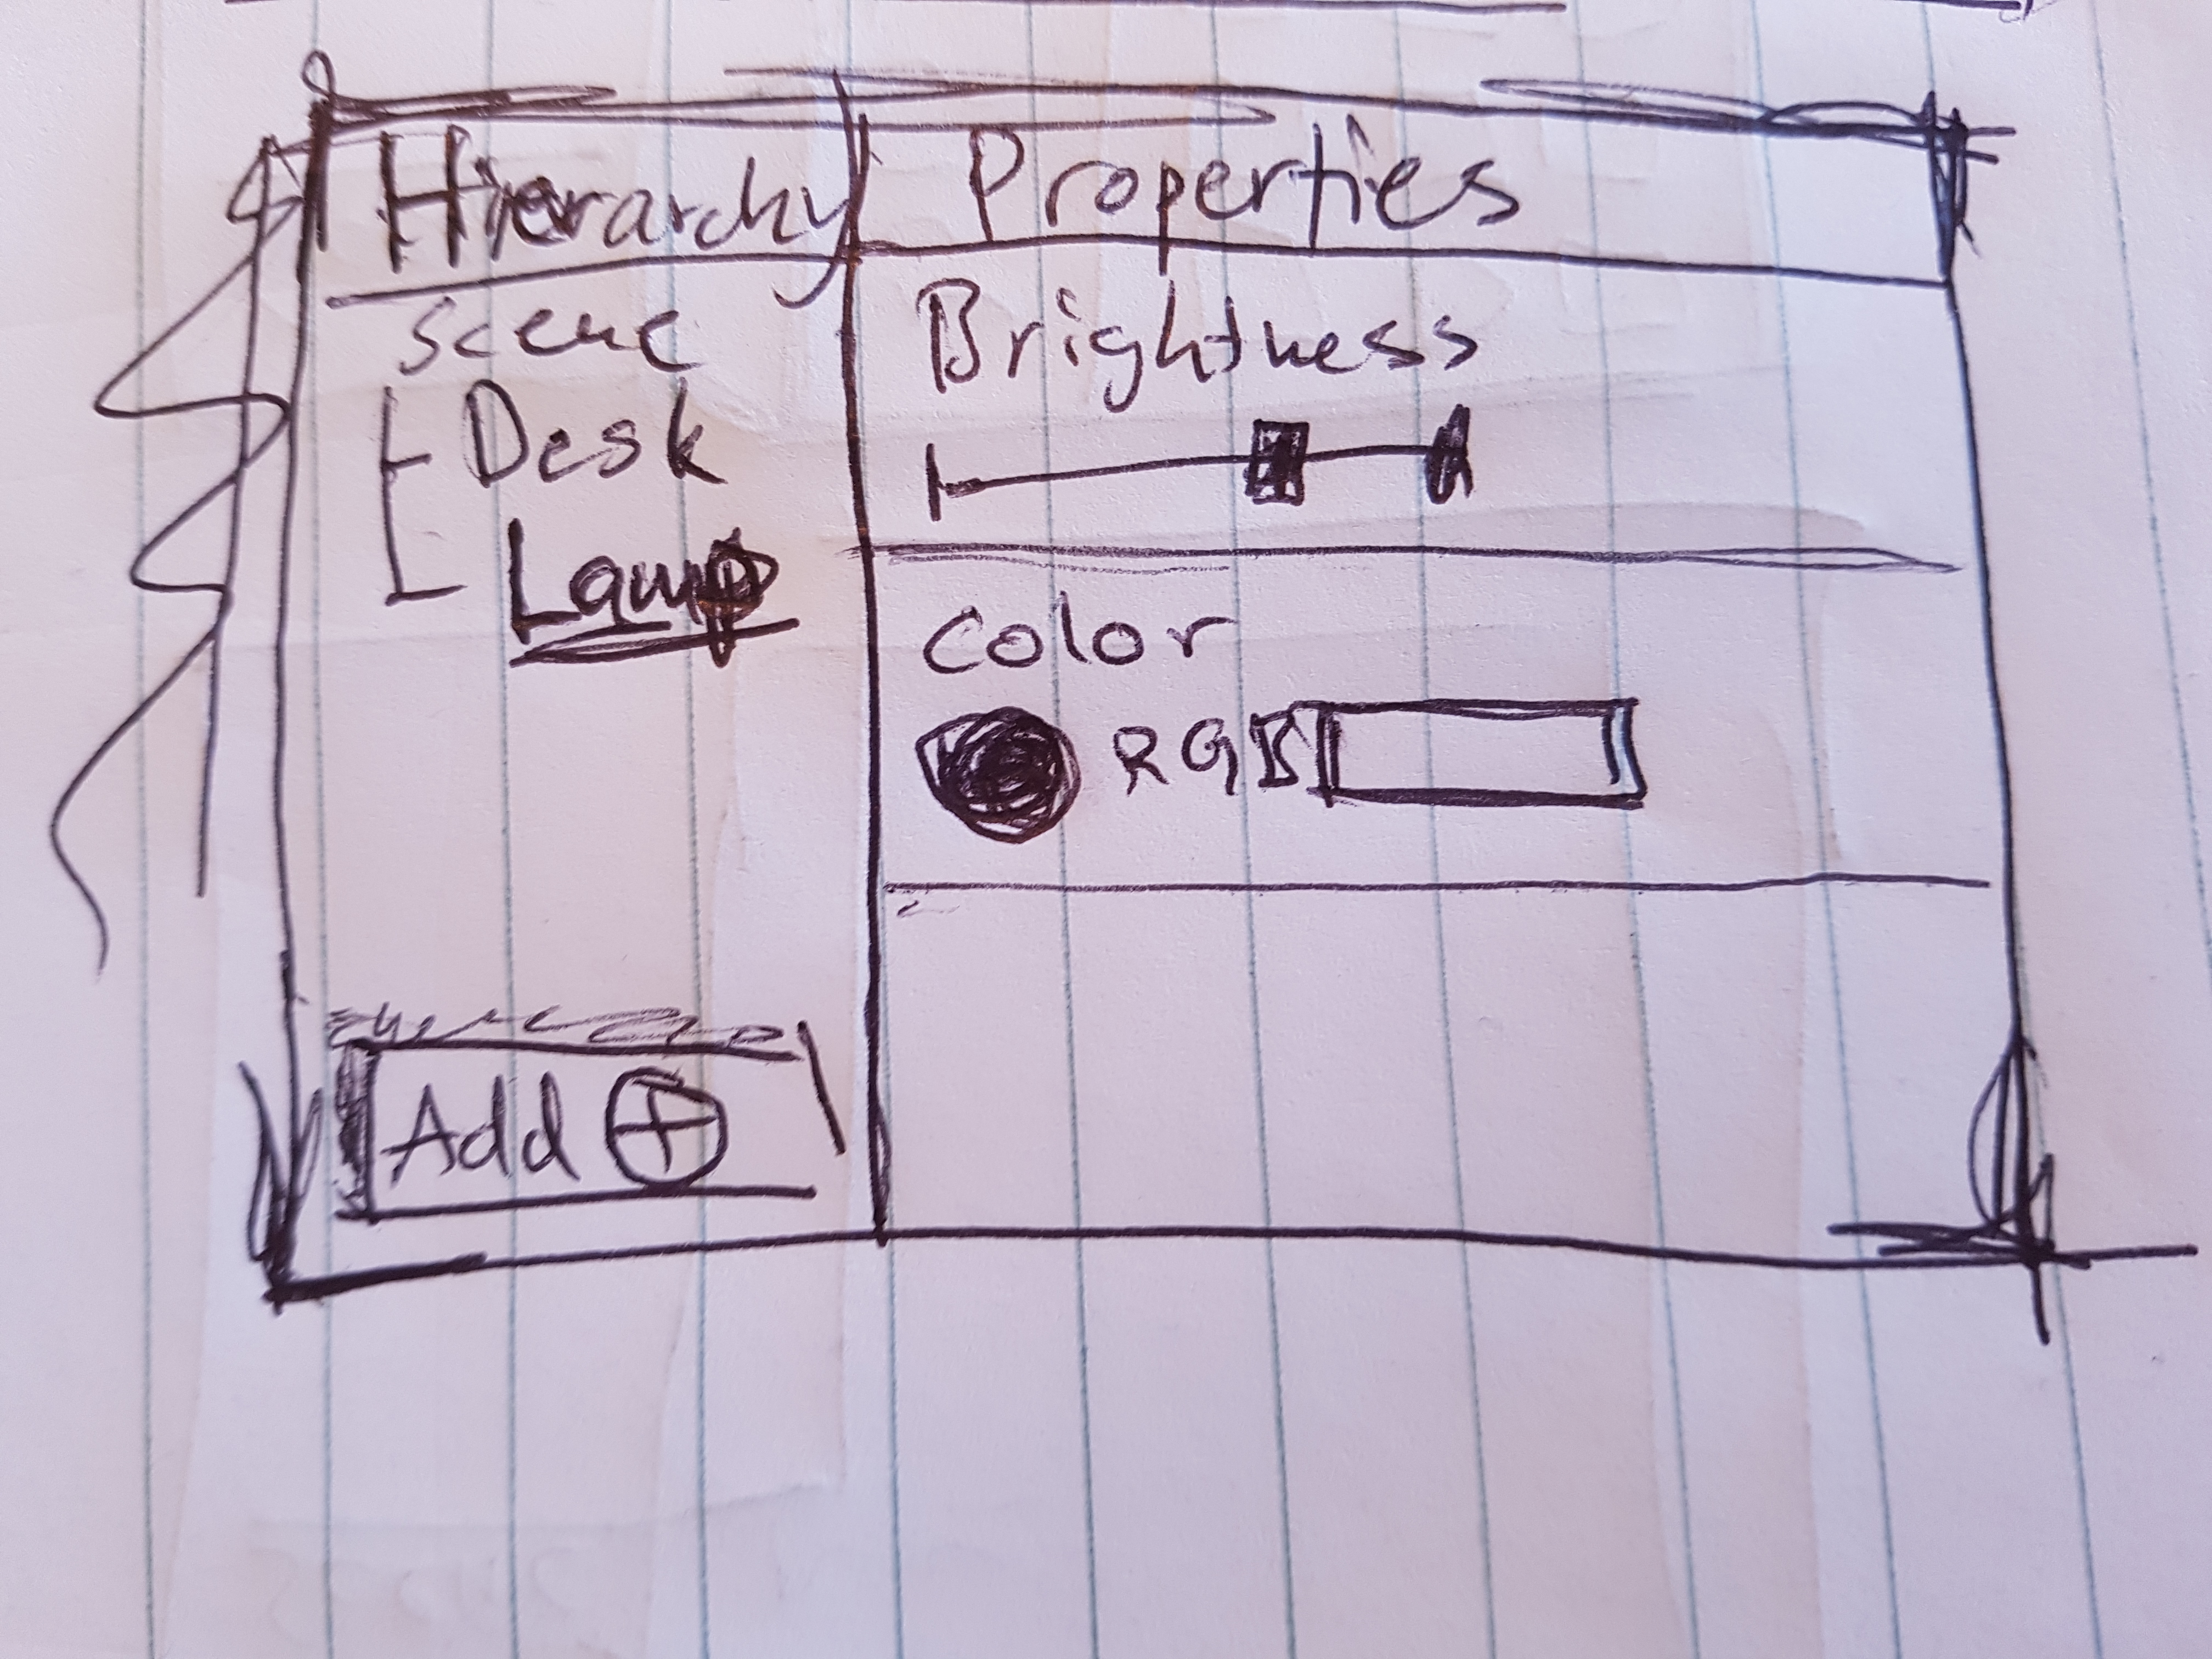
\includegraphics[width=.8\linewidth]{lo-fi/belt-props.jpg}
  \caption{A selection of objects that can be added to the VE}
  \label{fig:lofi:belt-ui:add}
\end{subfigure}
\caption{Paper sketches of the primary UI of the tool: Belt UI}
\label{fig:lofi:belt-ui}
\end{figure}

%% ********* BELT UI IMAGES **********

\begin{figure}
\begin{subfigure}{.5\textwidth}
  \centering
  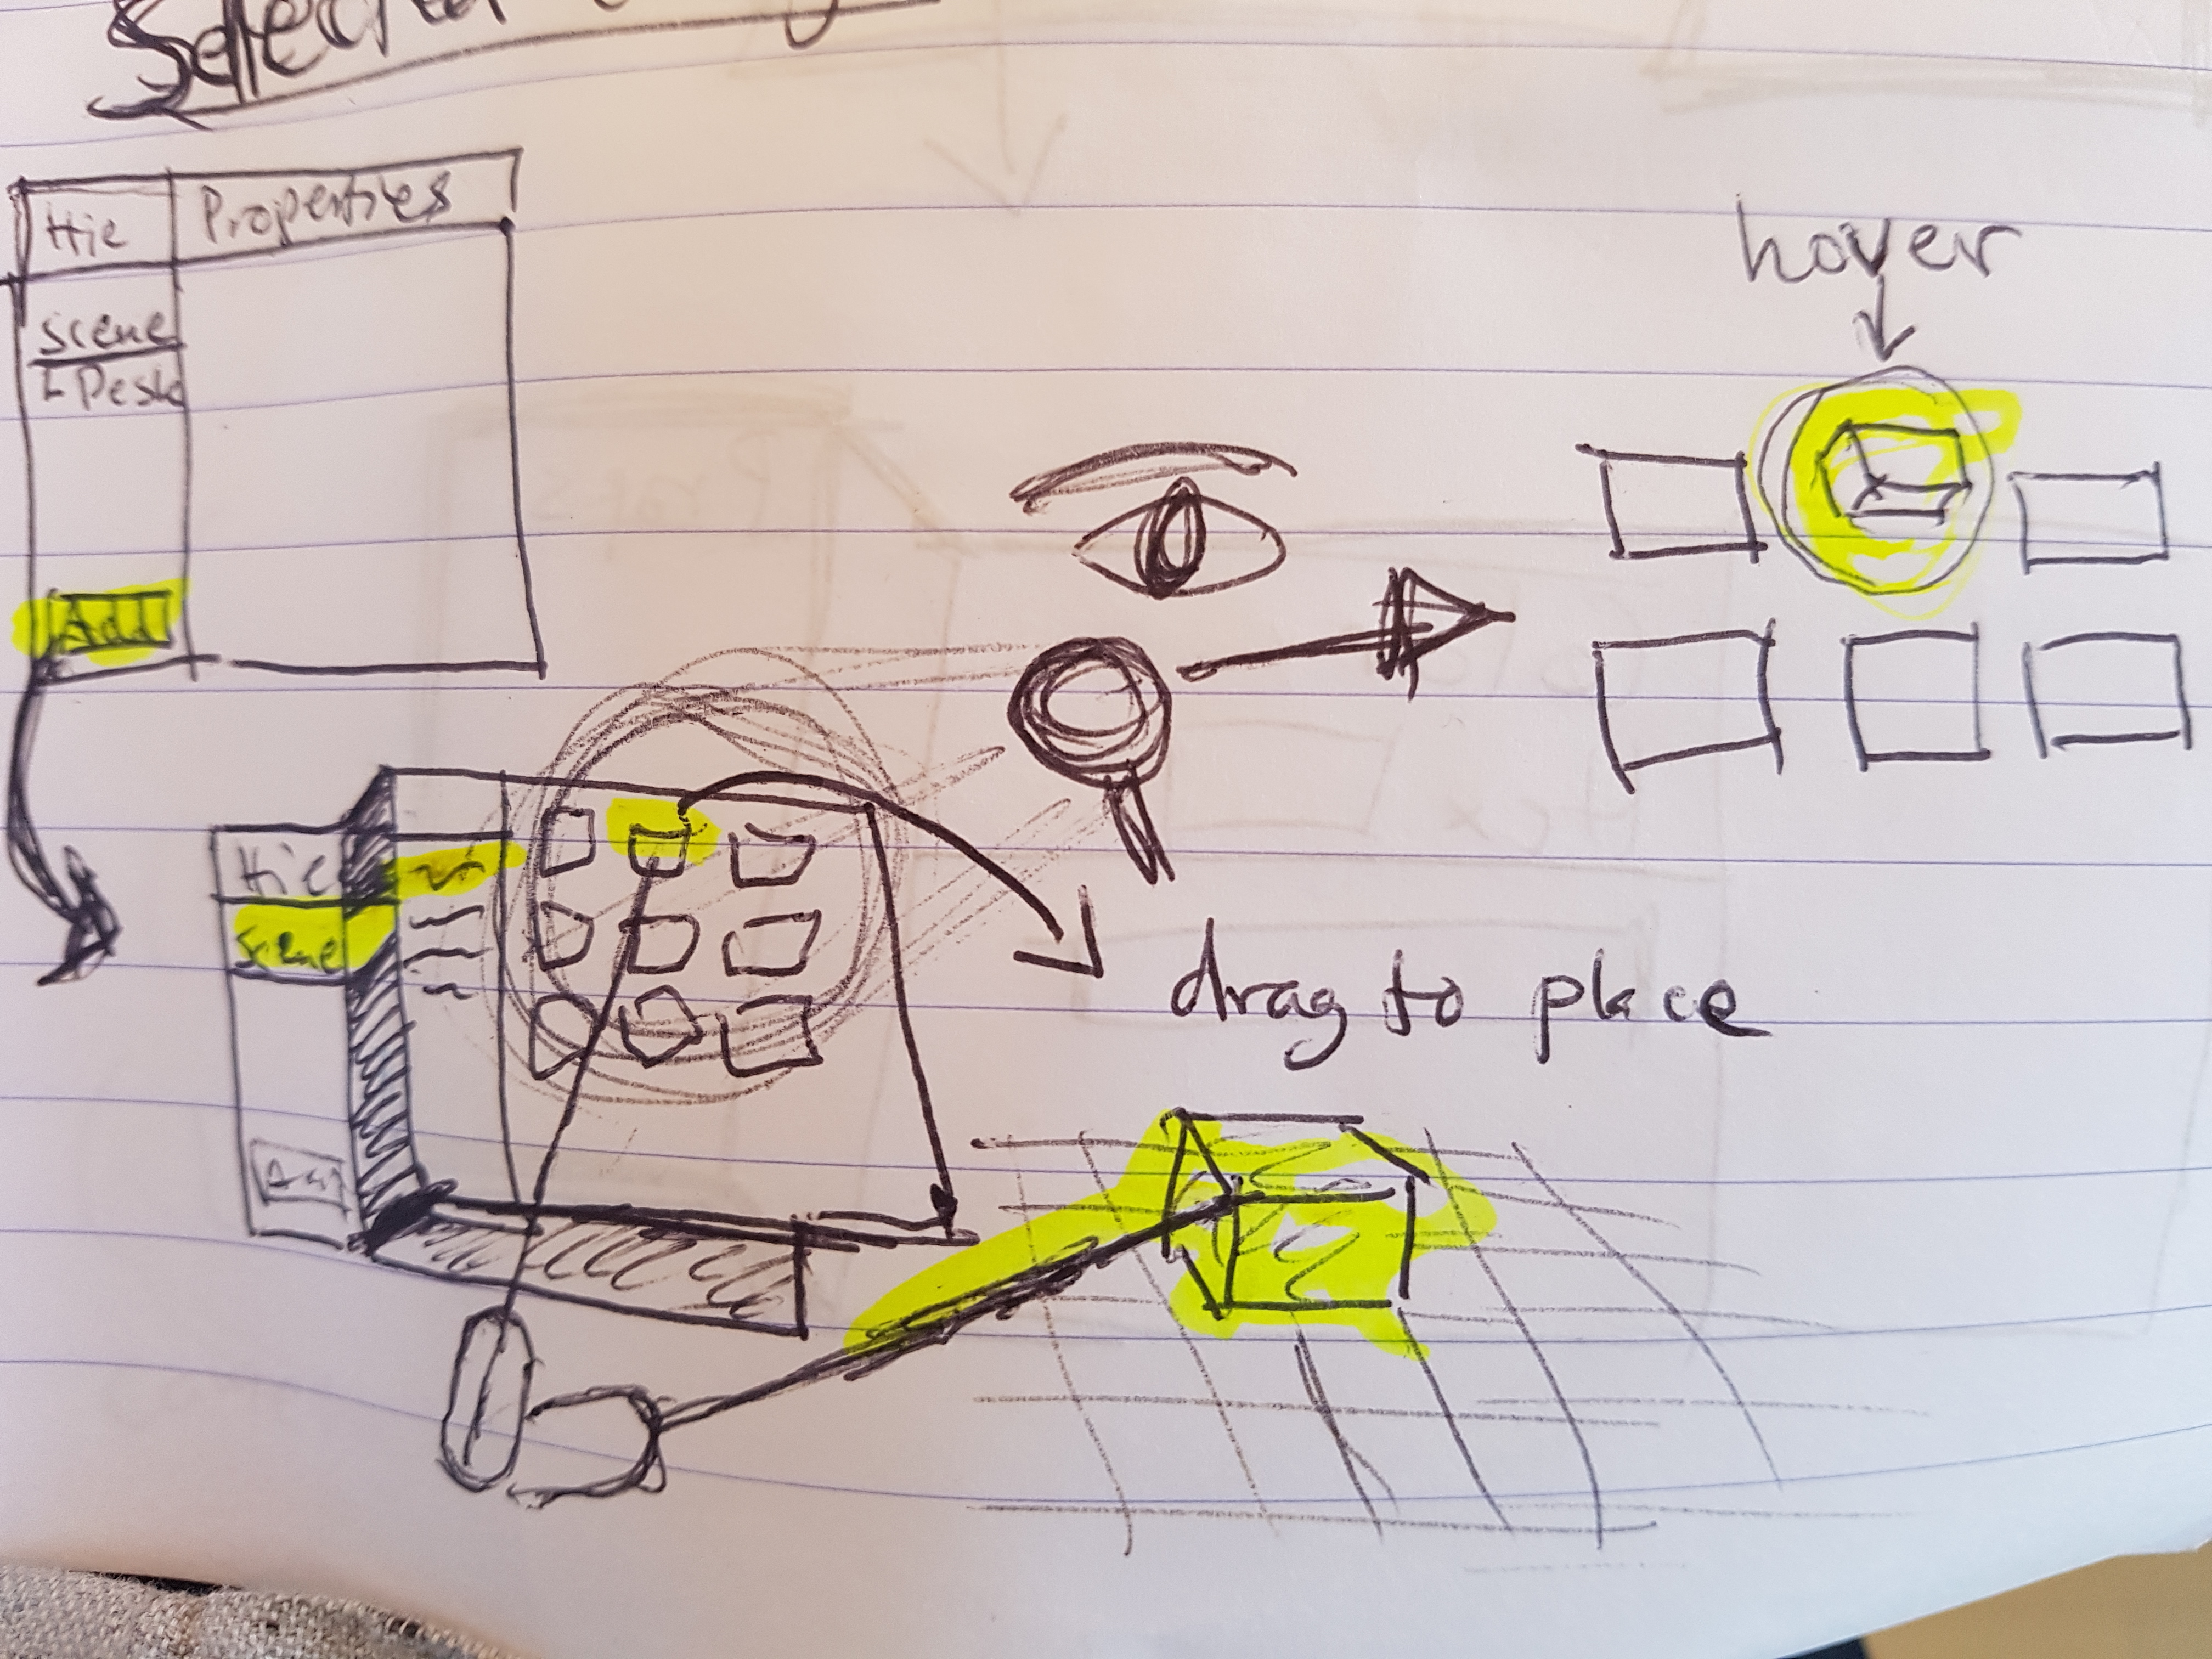
\includegraphics[width=.8\linewidth]{lo-fi/add-object.jpg}
  \caption{Properties of a selected object in the belt UI}
  \label{fig:lofi:object:add}
\end{subfigure}%
\begin{subfigure}{.5\textwidth}
  \centering
  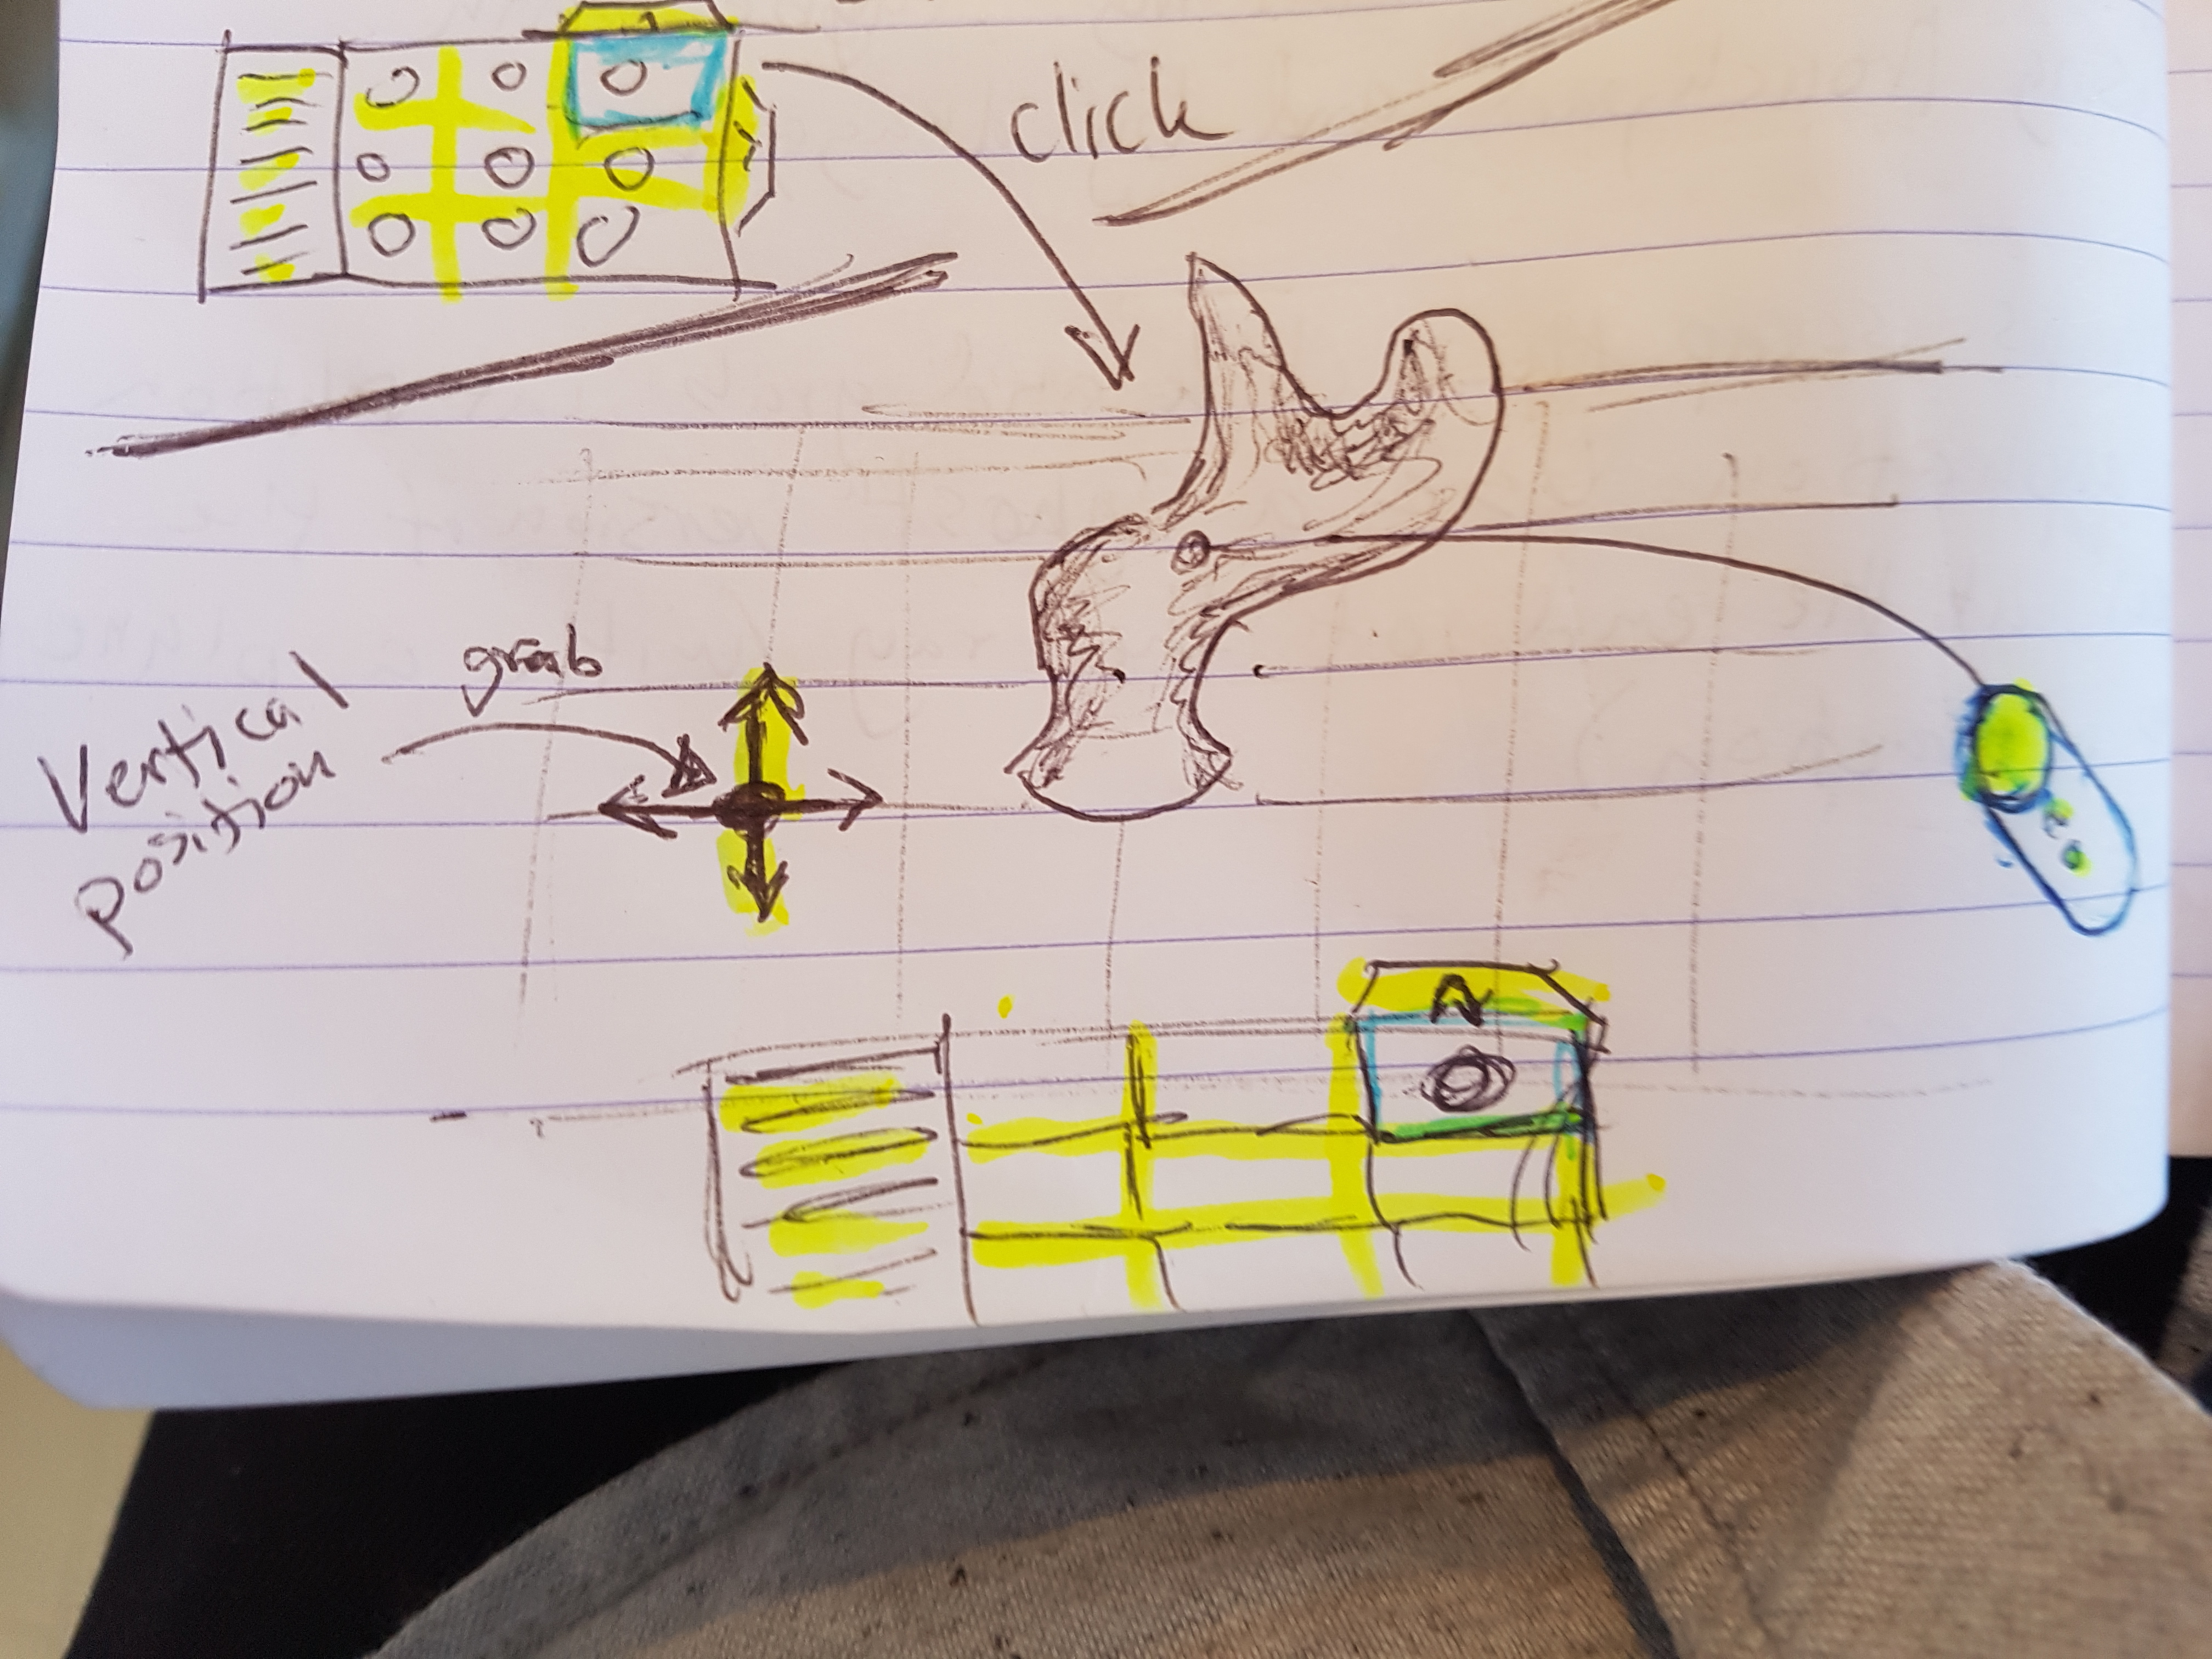
\includegraphics[width=.8\linewidth]{lo-fi/move-object.jpg}
  \caption{A selection of objects that can be added to the VE}
  \label{fig:lofi:object:move}
\end{subfigure}
\caption{Paper sketches of the primary UI of the tool: Belt UI}
\label{fig:lofi:object}
\end{figure}


\subsubsection{User Interface Selectors}
\label{result:lofi:selector}
A selector UI (building from work in section \ref{theory:toolsandtech:selector}) is used to manipulate and interact with objects. As seen in Figure \ref{fig:lofi:fov:selector}, the selector appears next to an object that has been selected and offers actions that are targeted to the selected object. The UI is designed as a pie-menu (Figure \ref{fig:lofi:selector:select}) that grants the oppertunity one level of sub-menus (Figure \ref{fig:lofi:selector:submenu}), similar to the interface of HoloSketch which is described in section \ref{relatedwork}. The selector UI is accessed through the touchpad on the controller (for hardware specs, see section \ref{theory:hardware:controllers}), but is visible as a part of the VE, unlike the interface in HoloSketch which hides all other elements and objects.

%% ********* SELECTOR IMAGES **********

\begin{figure}
\begin{subfigure}{.5\textwidth}
  \centering
  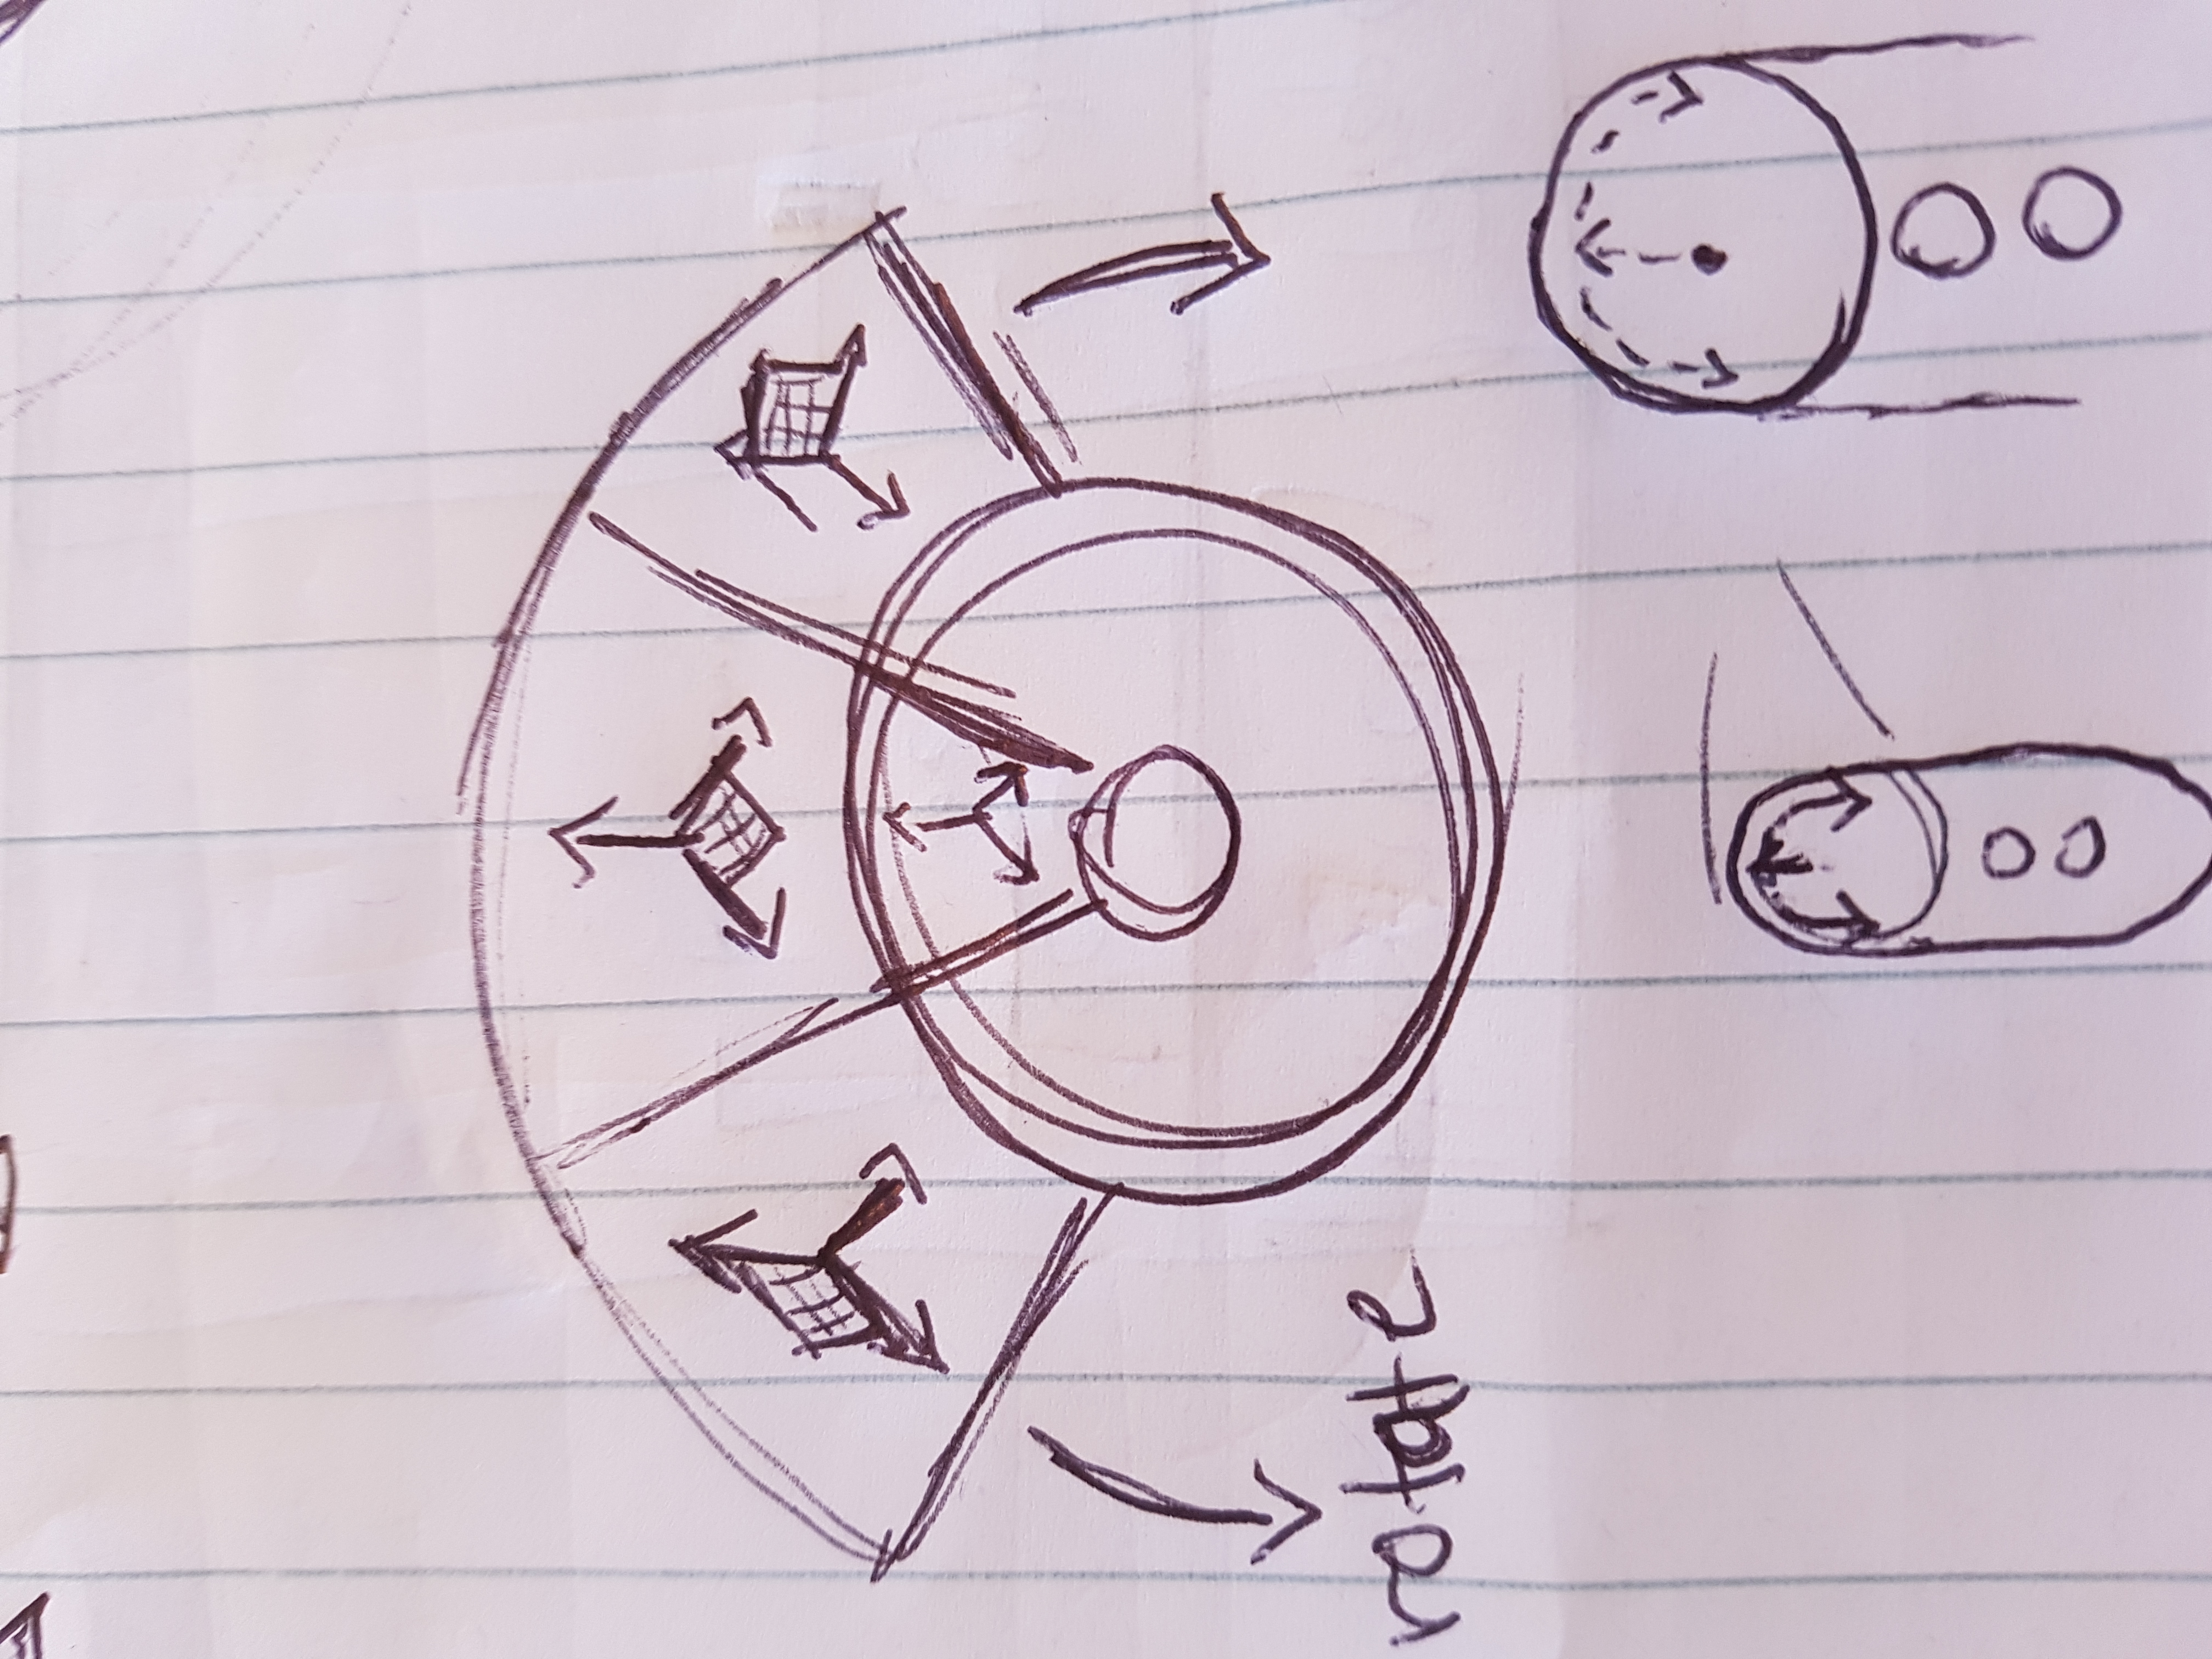
\includegraphics[width=.8\linewidth]{lo-fi/selector-submenu.jpg}
  \caption{Accessing a submenu of the selector}
  \label{fig:lofi:selector:select}
\end{subfigure}%
\begin{subfigure}{.5\textwidth}
  \centering
  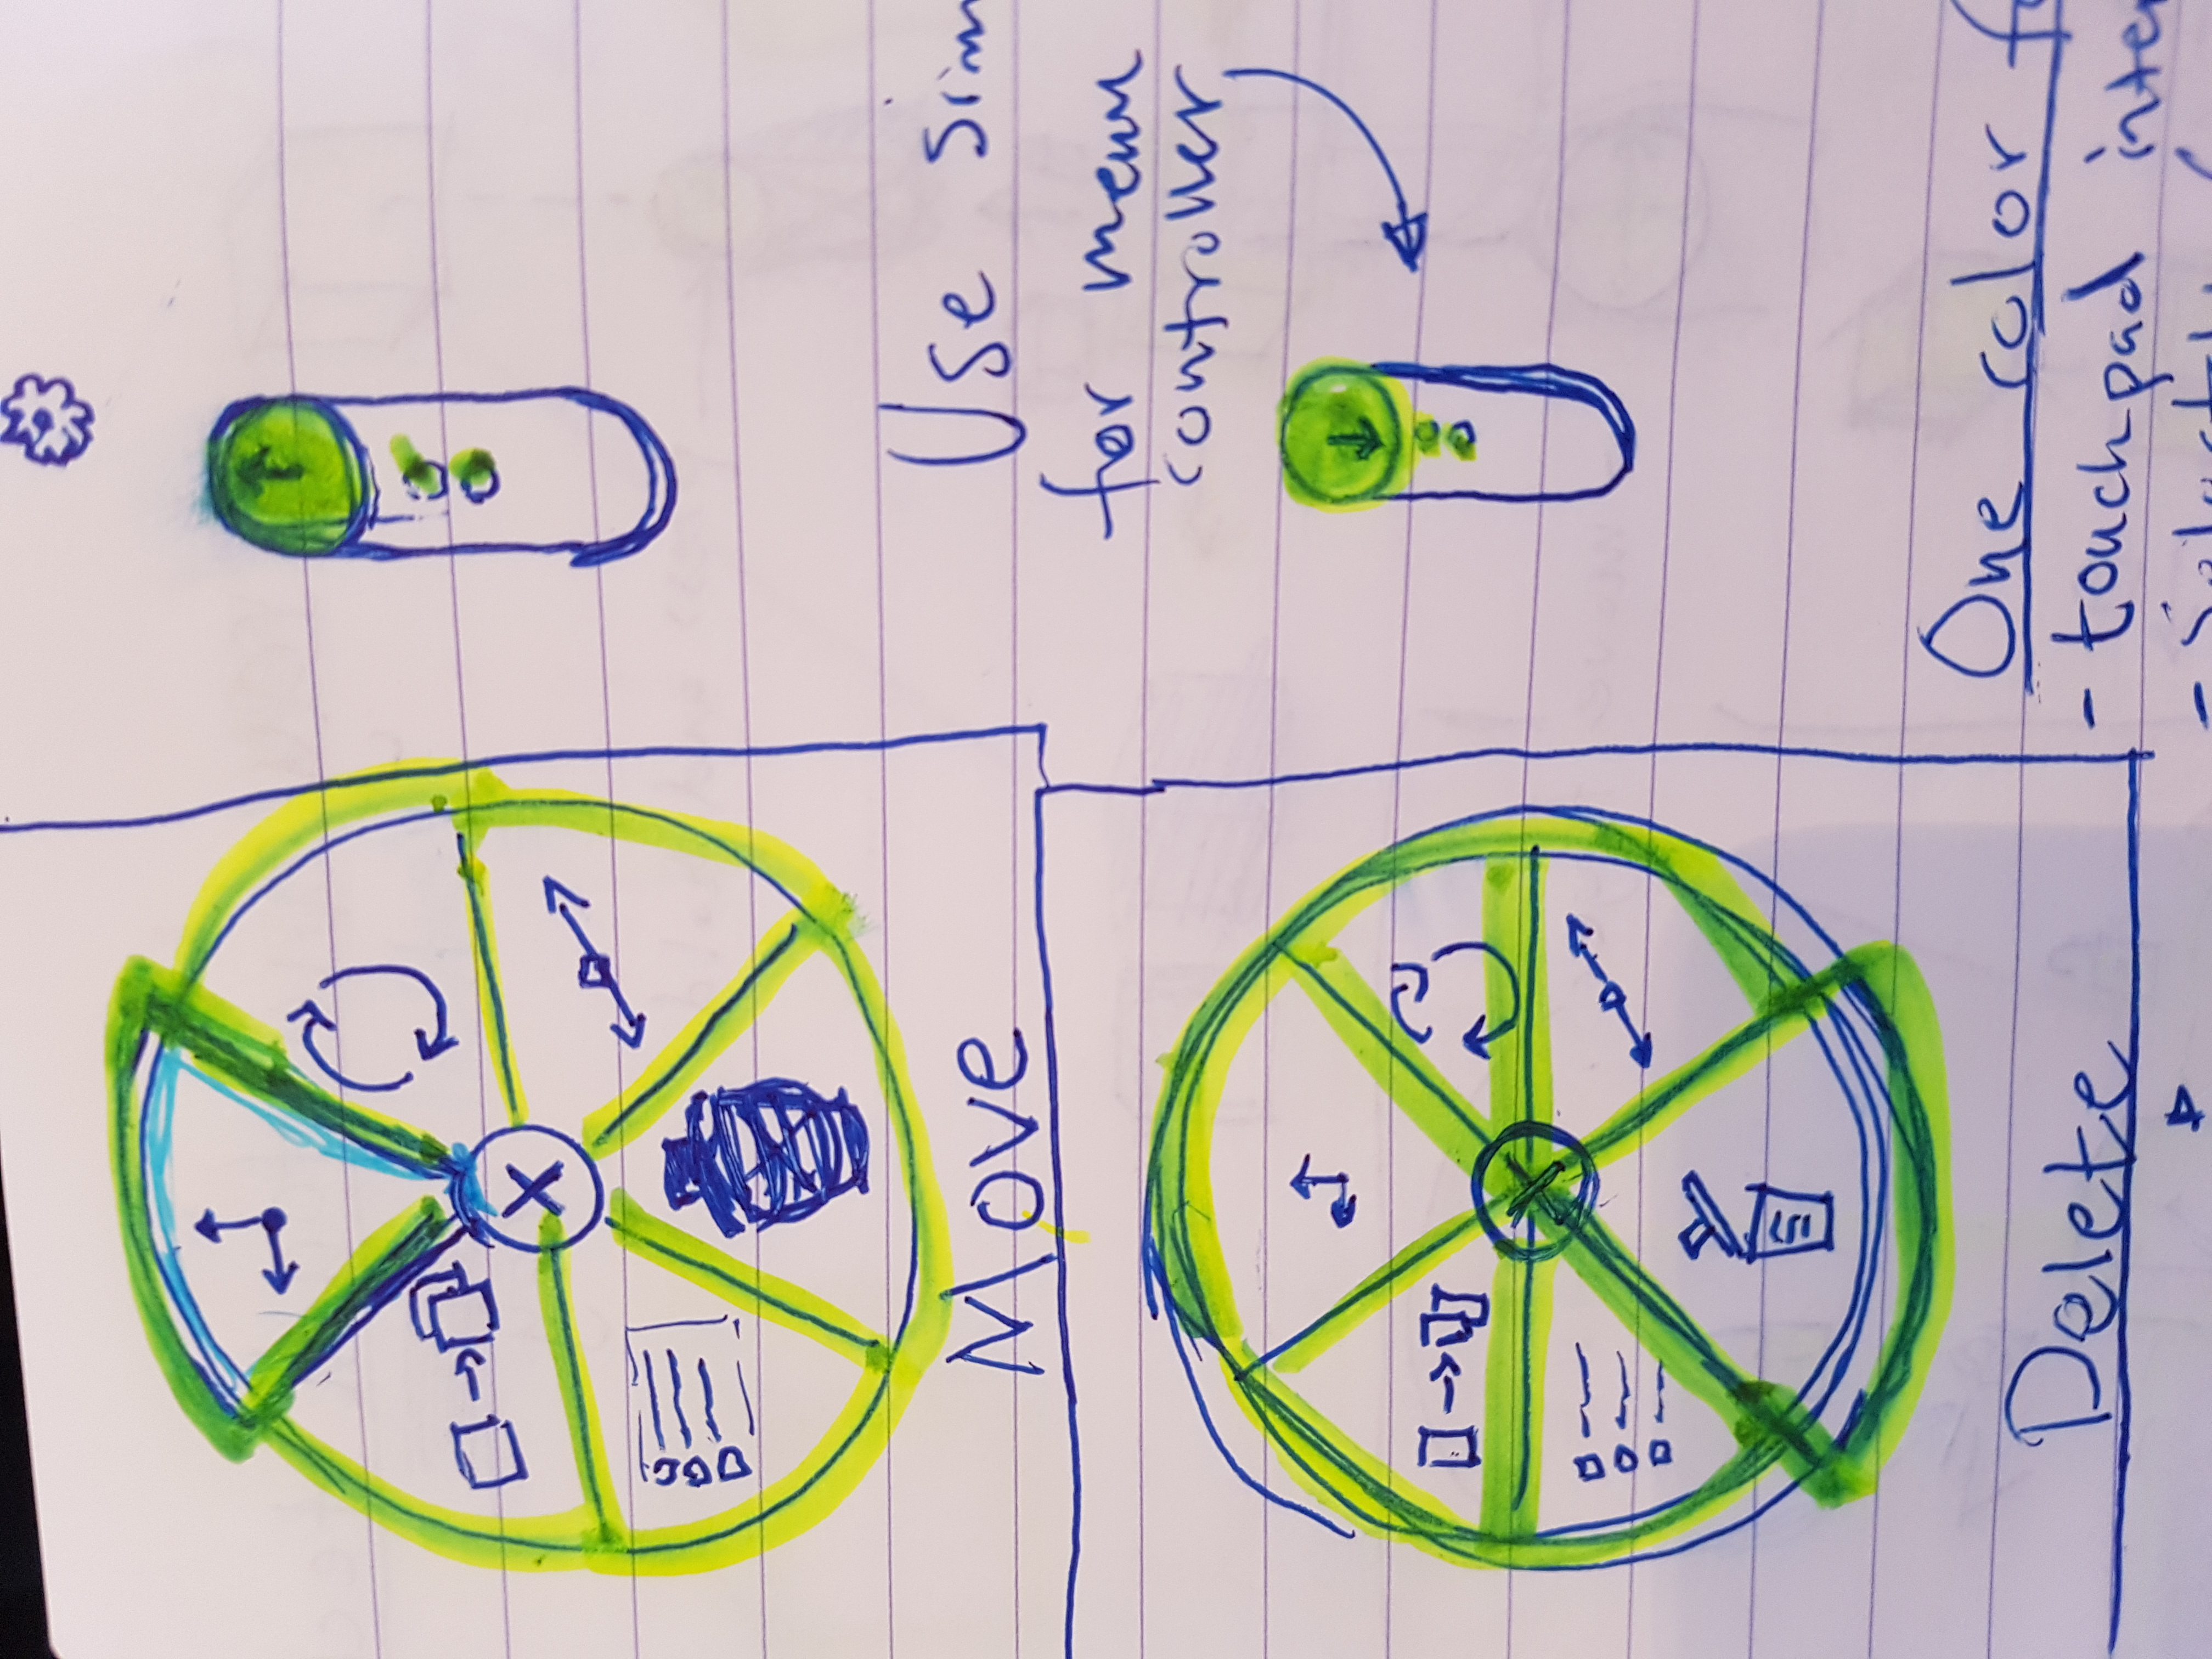
\includegraphics[width=.8\linewidth]{lo-fi/selector-select.jpg}
  \caption{selection in the selector}
  \label{fig:lofi:selector:submenu}
\end{subfigure}
\caption{Multilevel menu selector for objects}
\label{fig:lofi:selector}
\end{figure}

\subsubsection{Object selection and manipulation}
Interactions and sequences for selecting and manipulating objects (Figure \ref{fig:lofi:object}) are explained here as scenarios.
\begin{itemize}
  \item \textbf{Selecting an object} The user points the controller towards object, so that the raycast hits it. Then the user clicks the selection-button to select the targeted object.
  \item \textbf{Moving an object} When the user selects the object, a bounding-box becomes visible around the object along with three axis' and a grid (Figure \ref{fig:lofi:belt-ui:props}). By targeting the bounding-box and holding the selection-button the user can now use the raycast to position the object along the grid. If the user wants to move the object in the third dimension (that is not covered by the grid), grab the grid in a similar fashion and use the raycast to move. It's state is movable by default. Unless changed in the selector UI (section \ref{result:lofi:selector}), it can be moved straight away. The axis' of the grid can be changed using the selector UI.
  \item \textbf{Creating a new object} The user opens the Belt interface and selects the "New Component" button (in the hierarchy section), which displays a new view (Figure \ref{fig:lofi:object:add}). This view contains miniatures all objects that are avaliable to the user. The user finds the desired object, grabs it by holding the selection-button and points in the world to deside its position. the object is represented as a halv-transperant version of itself, and is placed by releasing the selection-button.
  \item \textbf{Duplicating an object} The user selects the object thats desired for duplication then opens the selector UI, then selects the 'Duplicate' option. The menu closes and the user points the ray-cast toward the grid of the original object. An identical half-transperant object appears at the end of the ray, onto to the grid. When the user is satisfied with the position, the selection-button is pressed to create the object in the selected location.
  \item \textbf{Properties of an object} The user opens the Belt UI, then selects an object with the raycast. The selection can be made on the actual object or on the object name in the hierarchy in the UI. When an object is selected, all properties for this object is displayed in the right section of the Belt UI (Figure \ref{fig:lofi:belt-ui:props}). A new property can be added by selecting the "Add property" button.
\end{itemize}

%% ********* FIELD-OF-VIEW IMAGES **********

\begin{figure}
  \begin{subfigure}{.5\textwidth}
  \centering
  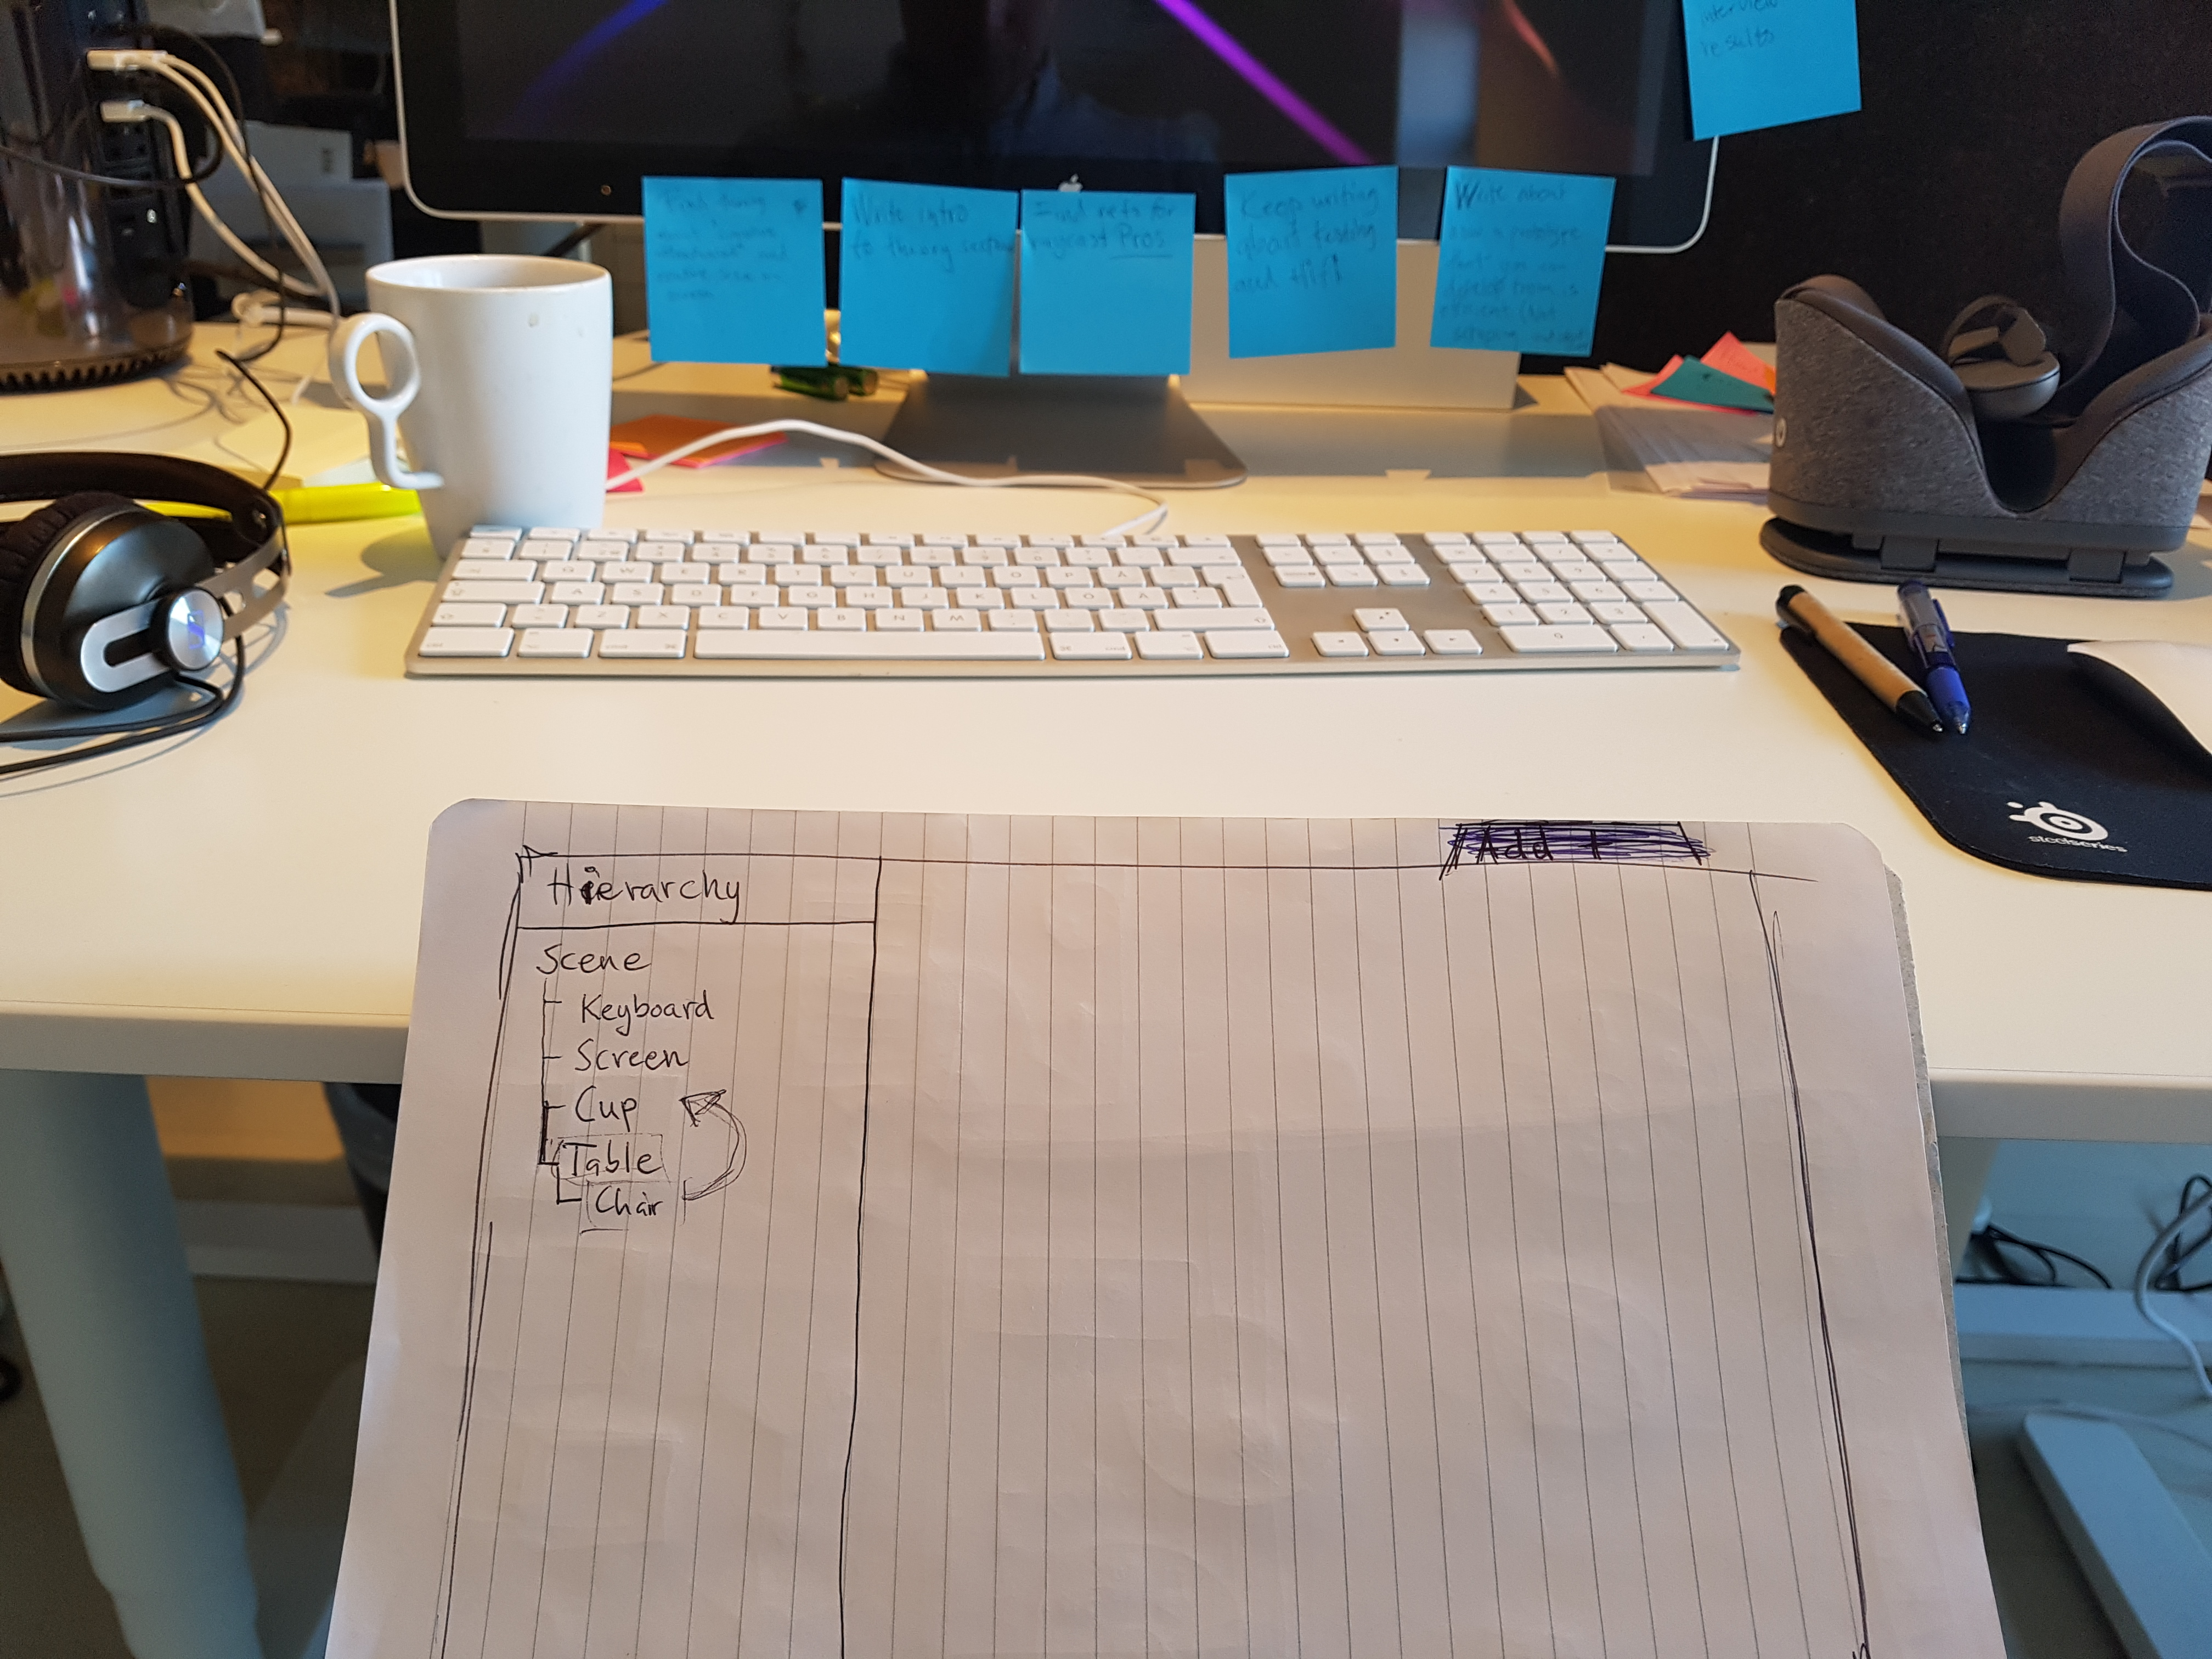
\includegraphics[width=.8\linewidth]{lo-fi/belt-perspective.jpg}
  \caption{Field of view for the user with the belt UI open}
  \label{fig:lofi:fov:belt-ui}
  \end{subfigure}%
  \begin{subfigure}{.5\textwidth}
    \centering
    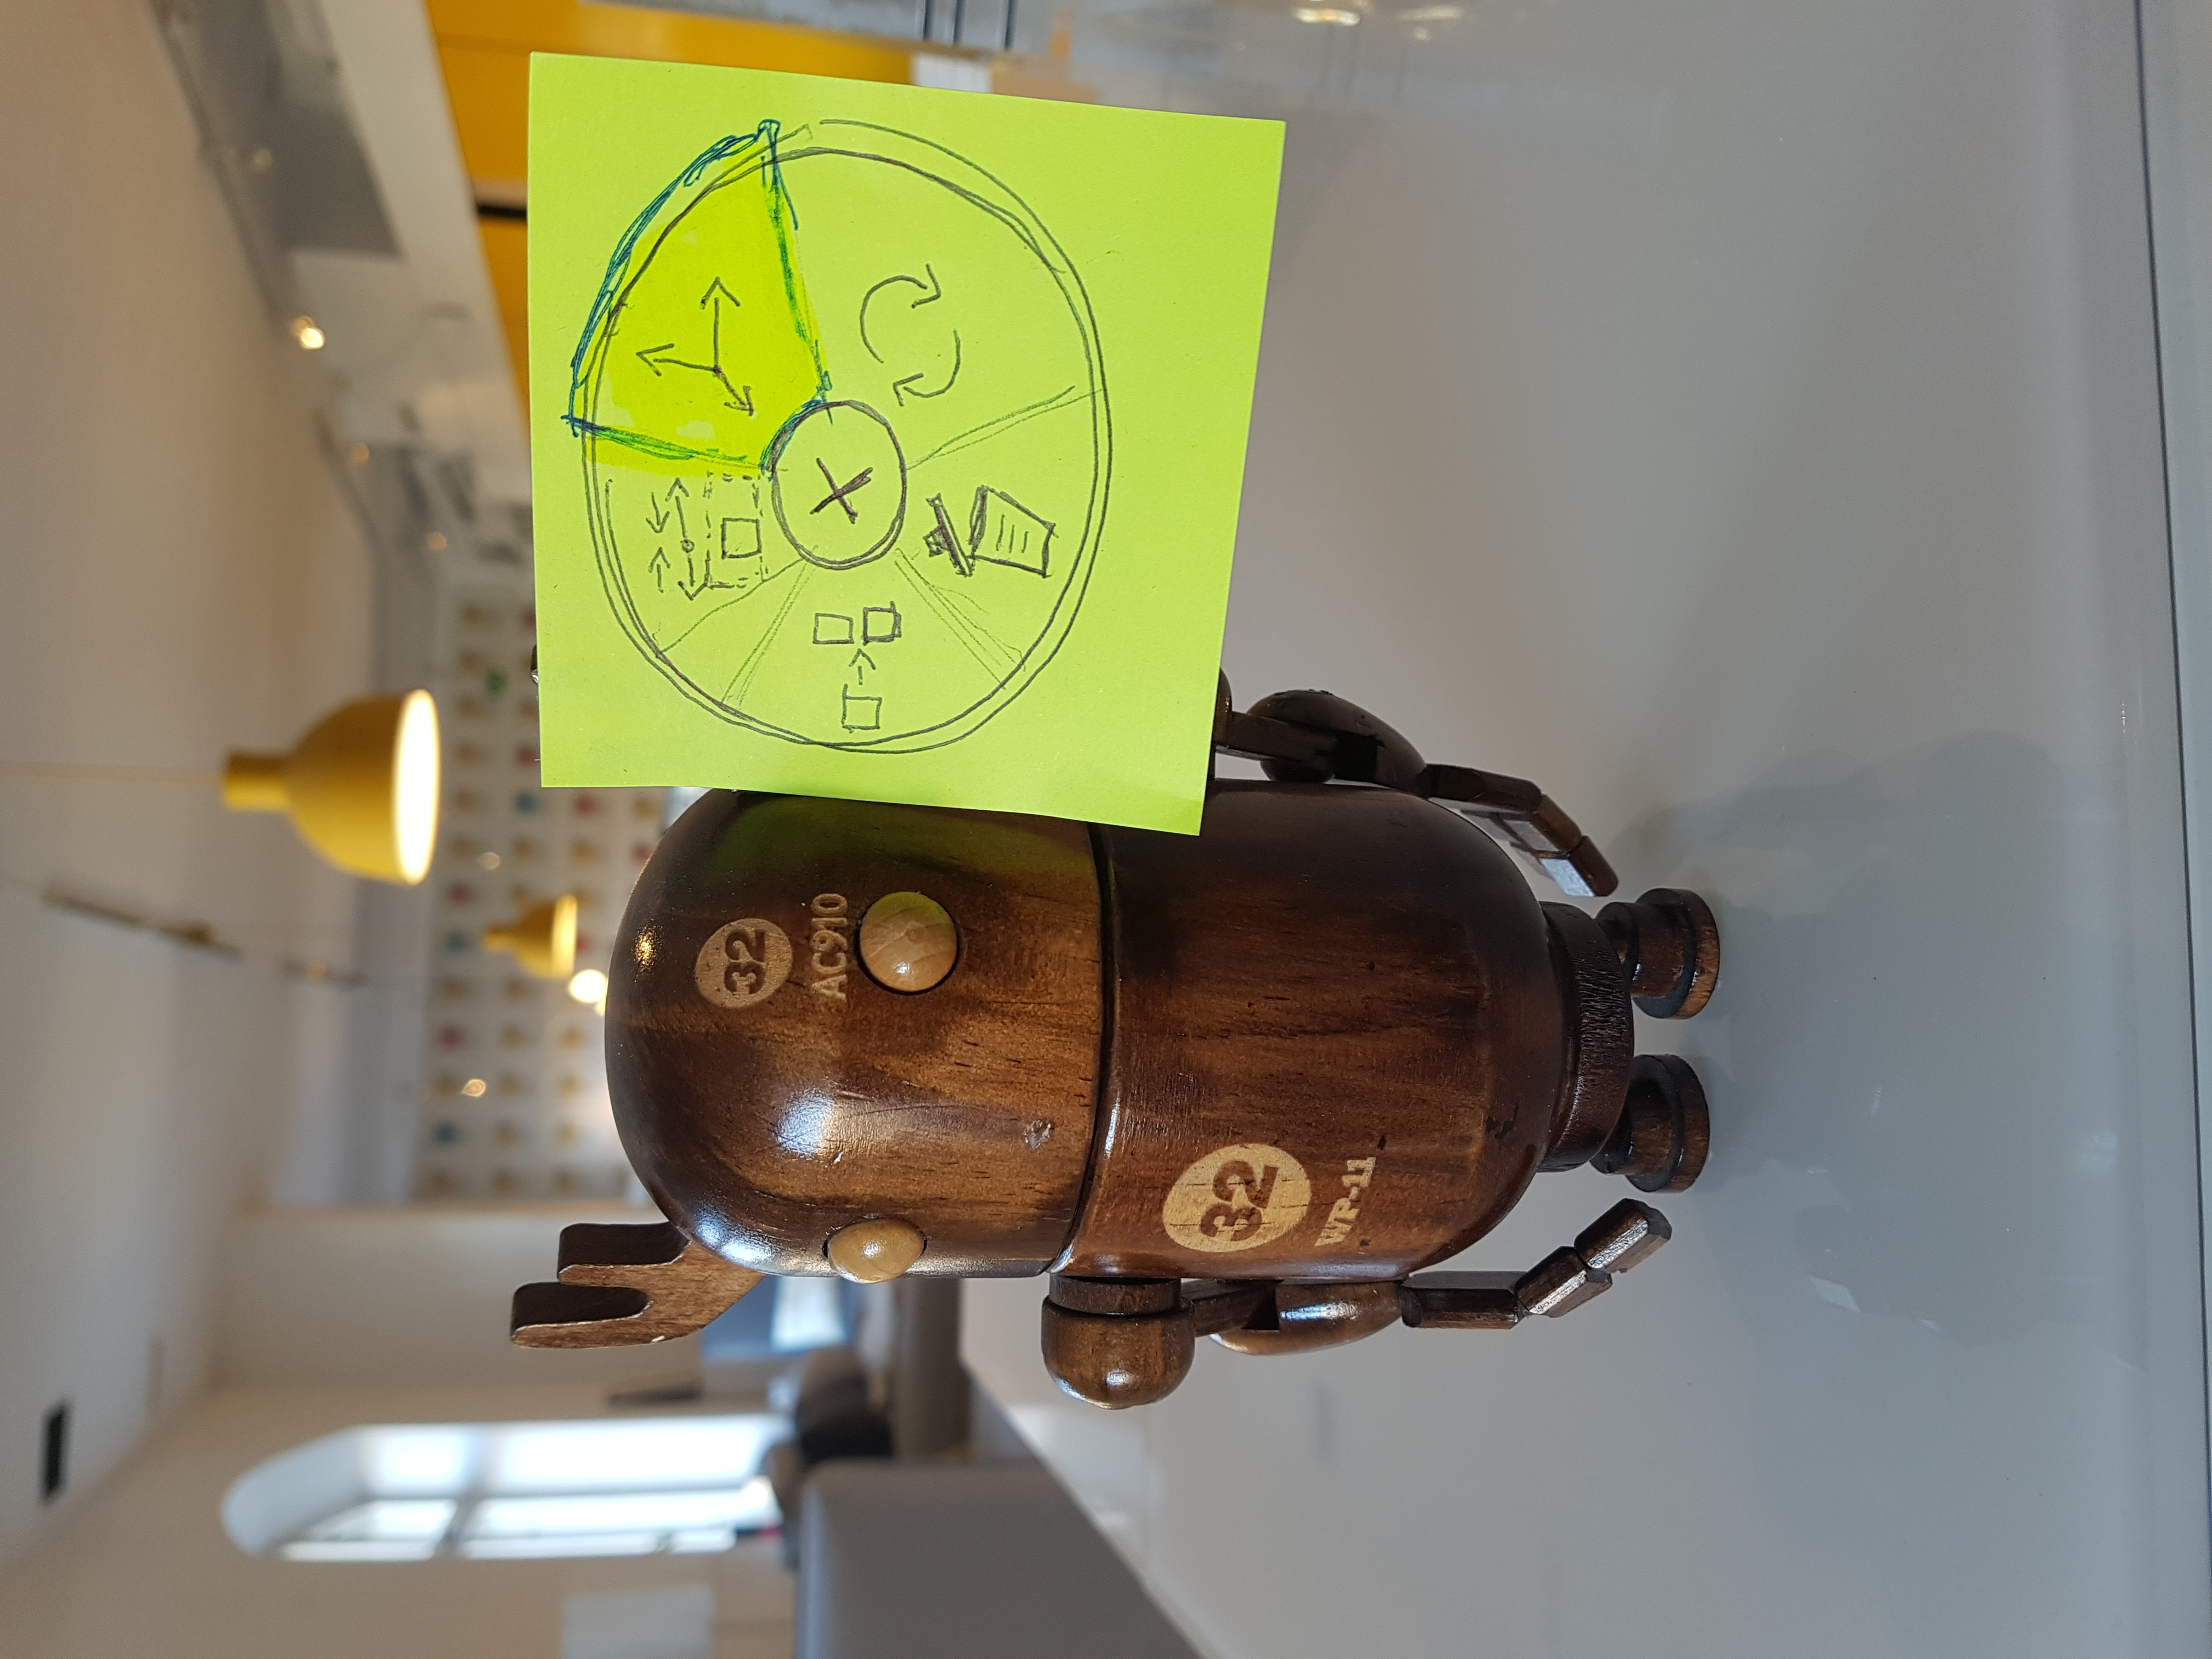
\includegraphics[width=.8\linewidth]{lo-fi/selector-perspective.jpg}
    \caption{Field of view for the user with a visible selector}
    \label{fig:lofi:fov:selector}
\end{subfigure}
\caption{Field of view for the user with different parts of the UI}
\label{fig:lofi:fov}
\end{figure}


\subsubsection{Tilt-Brush Tests}
Concepts that made it through initial testing were drawn in Tilt Brush (see Figure \ref{fig:lofi:tilt})  to visulize how perspectives and field of view works with the concepts in VR. Using the application, frames from different scenarios were sketched out, containing UI's, objects and other visual elements.

%% ********* TILT BRUSH SKETCHES **********

\begin{figure}
\begin{subfigure}{.5\textwidth}
  \centering
  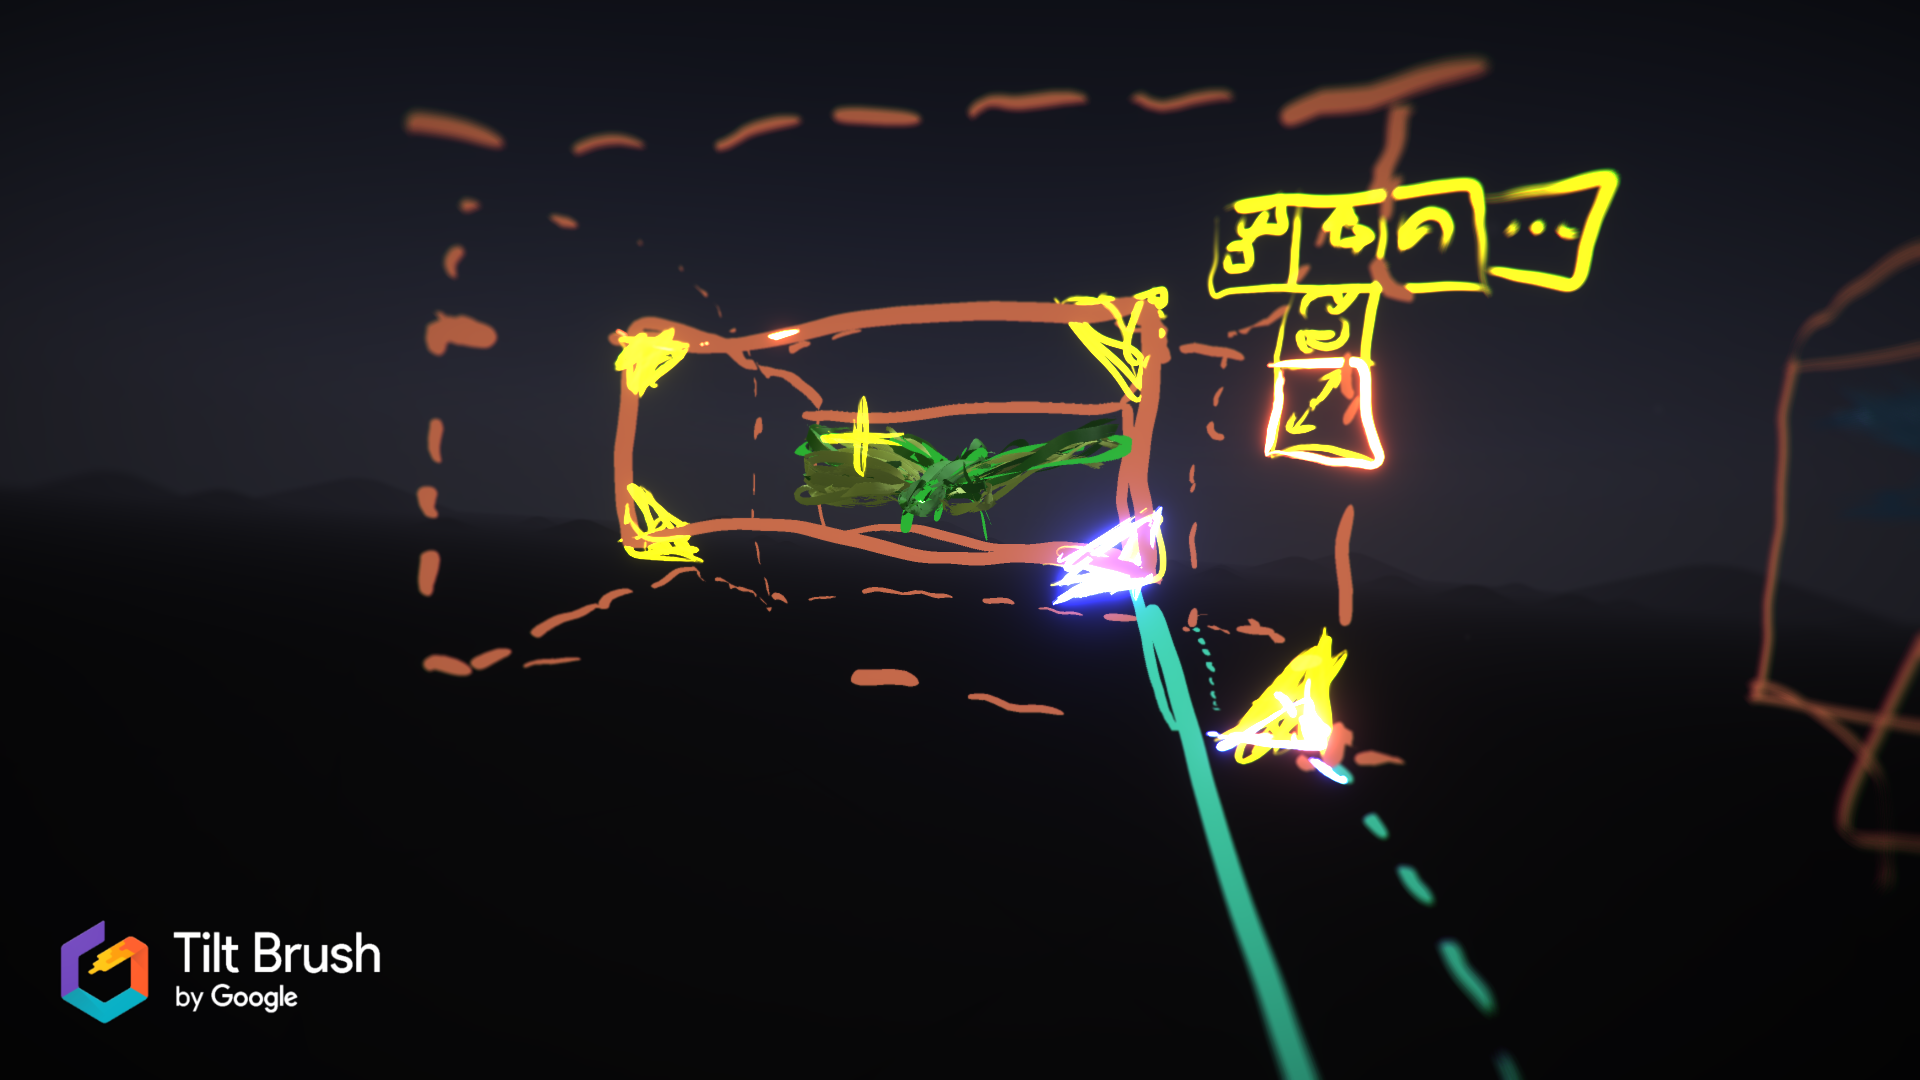
\includegraphics[width=.8\linewidth]{lo-fi/scalescenario3.PNG}
  \caption{A scale scenario where bottom right corner of a boundingbox is moved}
  \label{fig:lofi:tilt:scale3}
\end{subfigure}%
\begin{subfigure}{.5\textwidth}
  \centering
  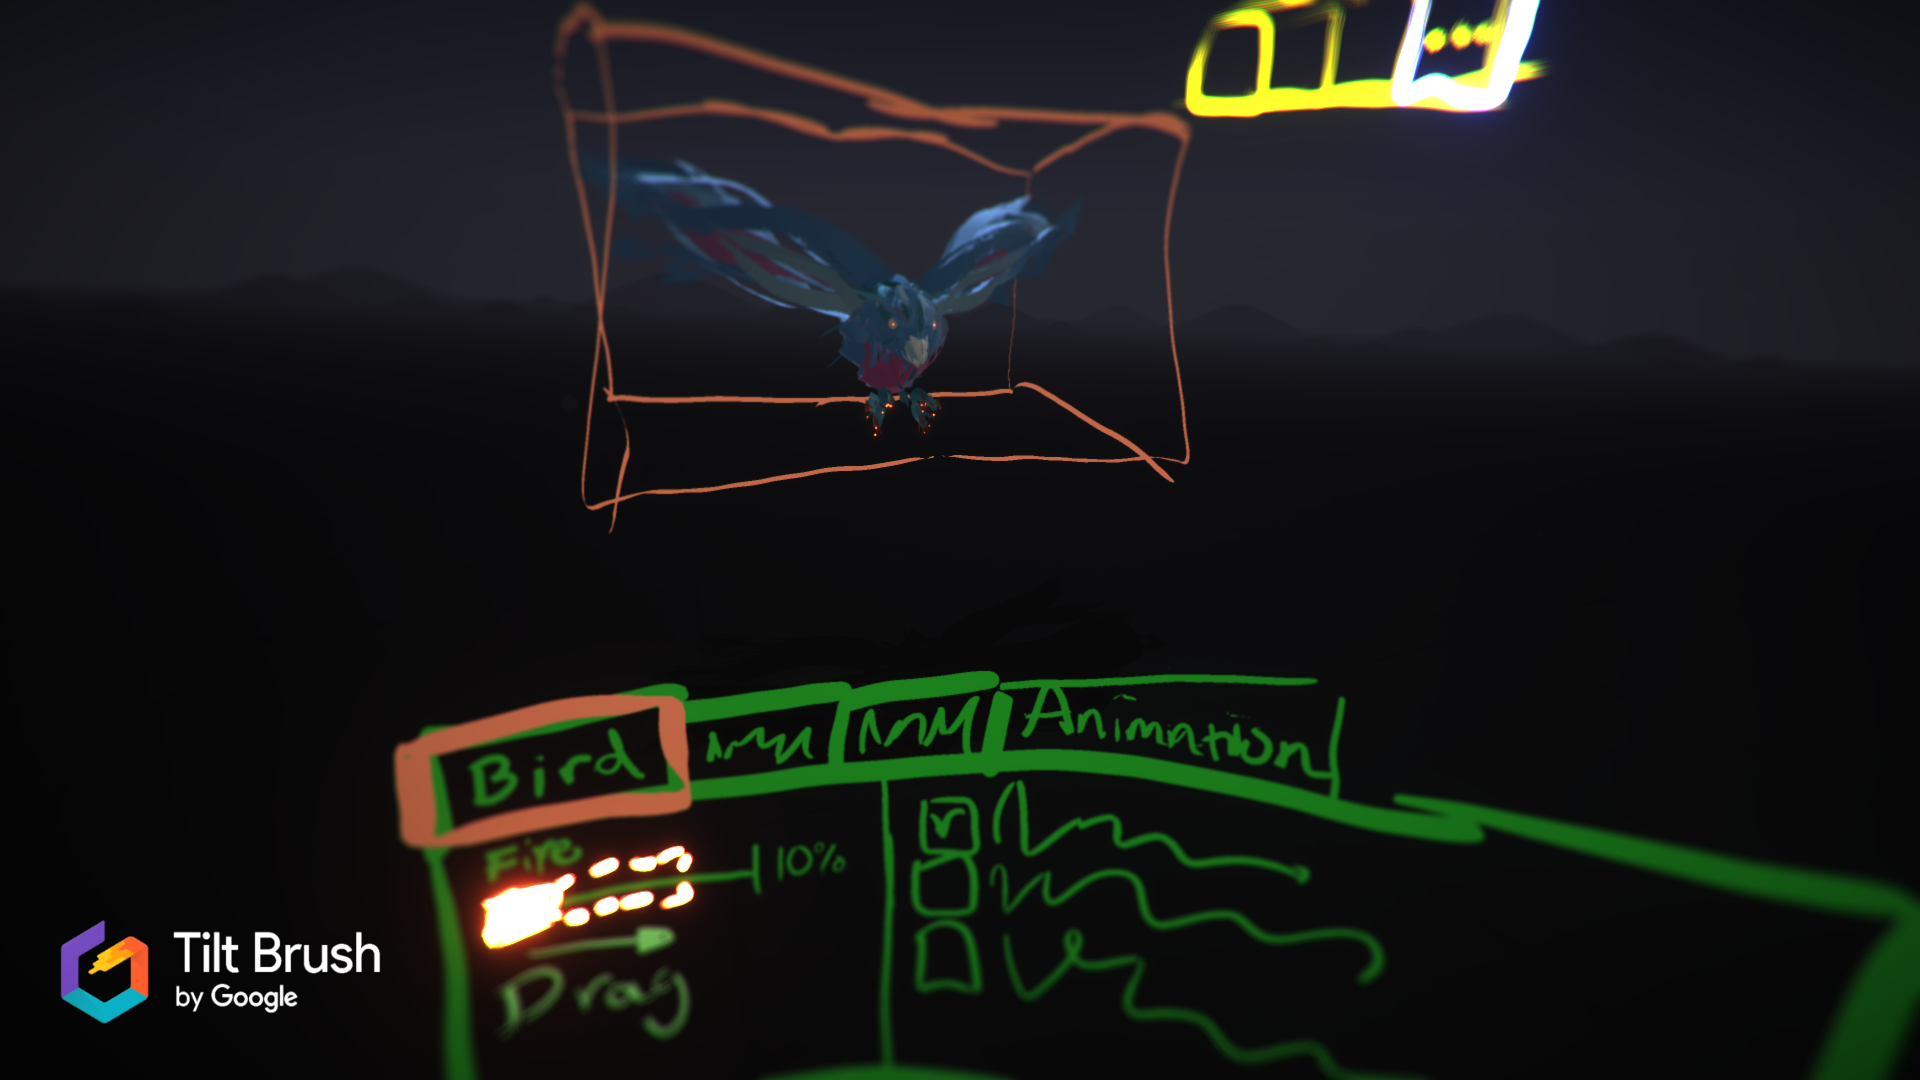
\includegraphics[width=.8\linewidth]{lo-fi/birdmenu2.PNG}
  \caption{Accessing properties of an object}
  \label{fig:lofi:tilt:passivemenu}
\end{subfigure}
\caption{Lo-fi sketches created in Tilt Brush }
\label{fig:lofi:tilt}
\end{figure}

\subsection{Hi-Fi Prototype}
Concepts and elements from the lo-fi prototypes were refined into hi-fi prototype. The hi-fi prototype is designed for mid-level and high-level VR devices, the interactive tests that followed were created for a HTC Vive. The prototype features elements from two main concepts/tools that were discovered.

The first is a tool for rough prototyping, as explained in section \ref{result:hifi:midlevel},that provides an intuitive and fast way to explore concepts without requiring previous scripting or VR development knowledge. This tool are to be used in the early stages of the experience design process (described in section \ref{intro:experiencedesign}). In later stages, when the concepts have been selected and are being developed, a tool acting as a test suite and with object manipulation is preferred. The hifi prototyp along with these concepts are presented in this section, which also covers results from user testing and concept evaluation.
\subsubsection{Main interface - Belt UI}
The main interface is designed for the users ergonomic position when seated, displayed from the hip of the user.(Figure \ref{fig:hifi:scenescreen}) The primary feature of this UI is to create new objects and place them in the world (Figure \ref{fig:hifi:belt-ui:add}) along with changing properties of objects (Figure \ref{fig:hifi:belt-ui:props}). Users interacts with the UI by pointing the raycast at an element and pressing the selection-button. The centered feature in this UI is the scene-hierarchy, from where objects can be selected and created. The users FOV will look like an extension of a work-bench (Figure \ref{fig:hifi:fov:belt-ui}), and can be accessed by pressing the application-button on the controller. The user can with direct manipulation (described in section \ref{theory:toolsandtech:direct}) position the screens in the UI according to their needs, to create the personal workstation.
%
% %% ********* BELT UI PROPERTIES AND OBJECTS **********
\begin{figure}
\begin{subfigure}{.5\textwidth}
  \centering
  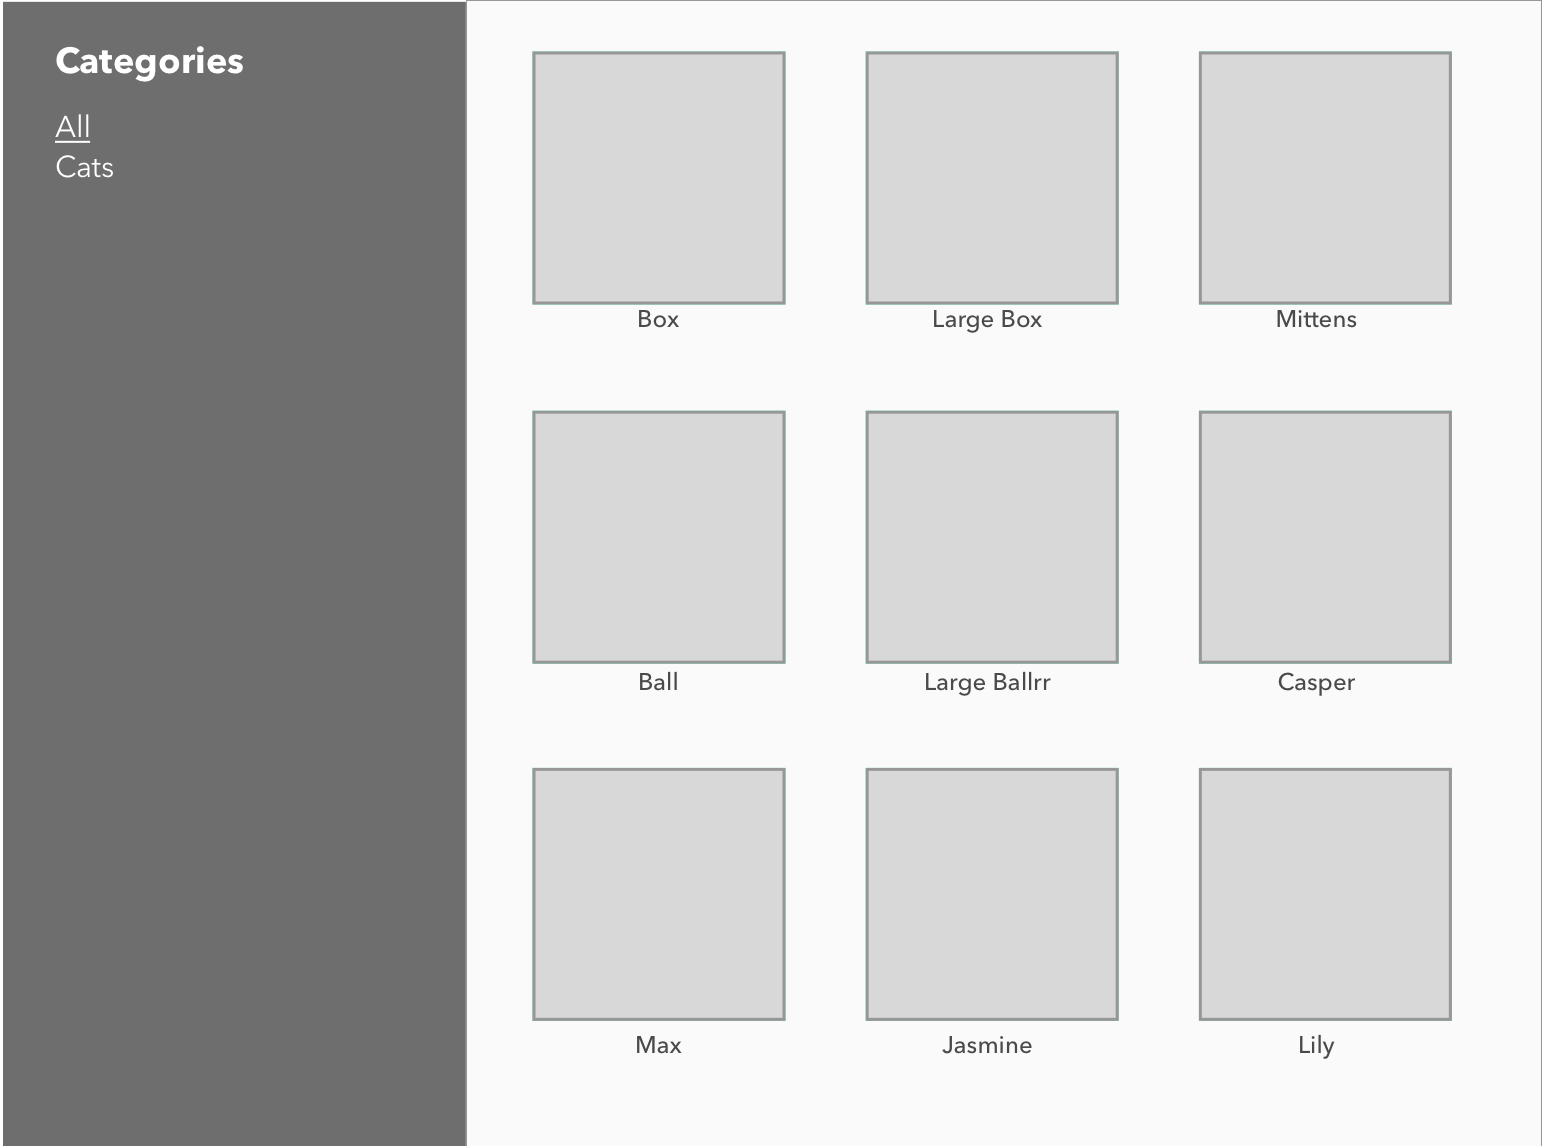
\includegraphics[width=.8\linewidth]{hi-fi/beltui_add.png}
  \caption{An interface for adding new objects to the VE}
  \label{fig:hifi:belt-ui:add}
\end{subfigure}%
\begin{subfigure}{.5\textwidth}
  \centering
  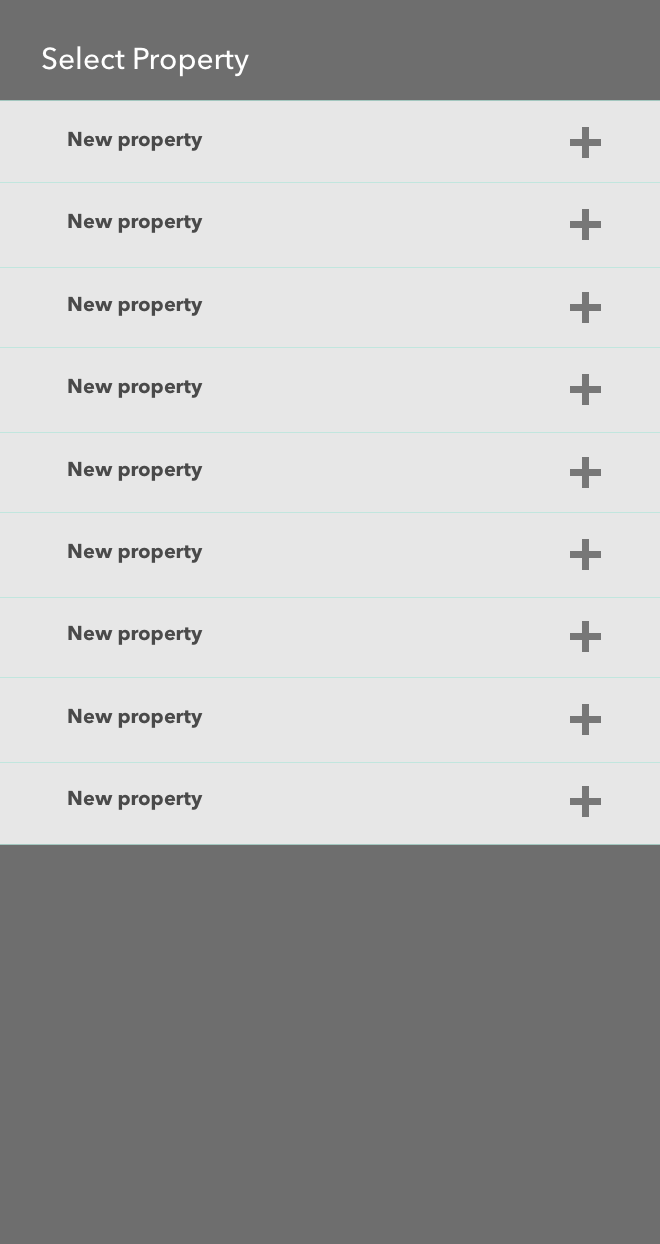
\includegraphics[width=.8\linewidth]{hi-fi/beltui_props.png}
  \caption{A list of properties that can be added to the selected object}
  \label{fig:hifi:belt-ui:props}
\end{subfigure}
\caption{Digital representations of object properties and selectable objects in the primary UI: Belt UI}
\label{fig:hifi:belt-ui}
\end{figure}

%% ********* BELT UI IMAGES **********

\begin{figure}
  \centering
  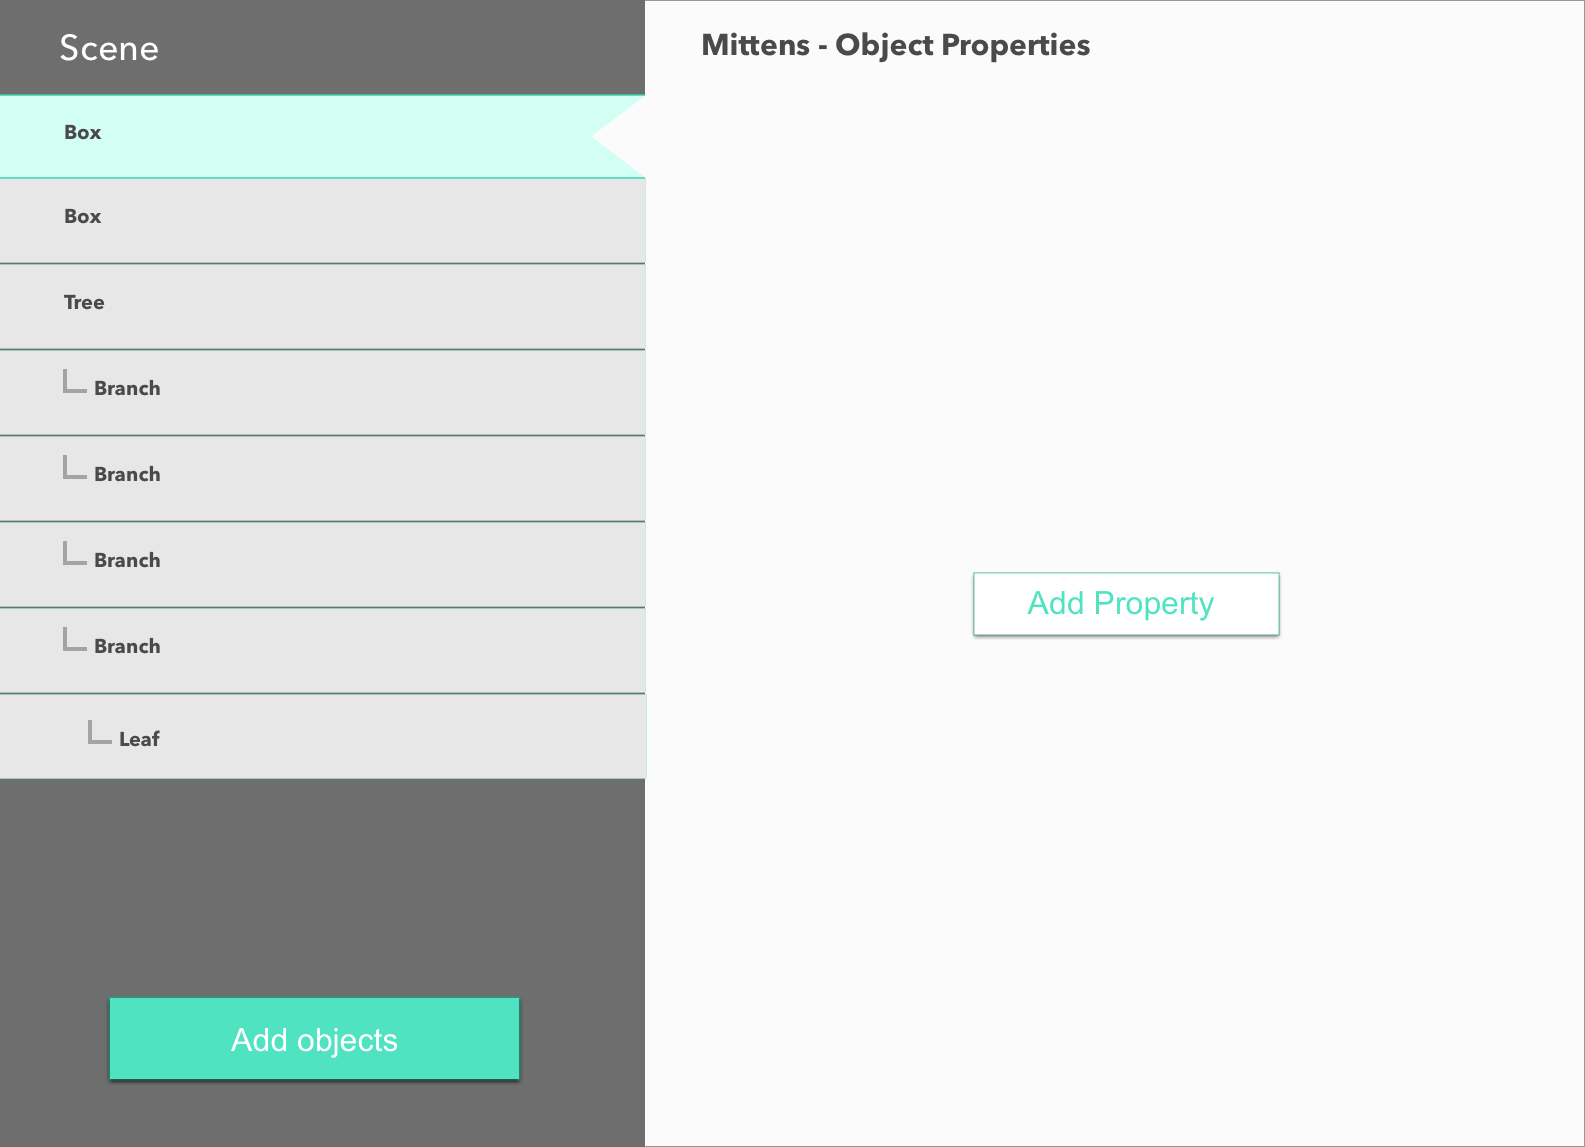
\includegraphics[width=.8\linewidth]{hi-fi/beltui_scene.png}
\caption{Digital representation of the scene and properties screen in the primary UI of the tool: Belt UI}
\label{fig:hifi:scenescreen}
\end{figure}

\subsubsection{User Interface - Object Manipulation}
\label{result:hifi:selector}
A secondary UI (figure \ref{fig:hifi:selector}) is placed on the touchpad of the primary controller as seen in Figure \ref{fig:hifi:fov:selector}, its primary use is manipulating selected objects. The UI is designed as a pie-menu (Figure \ref{fig:hifi:selector:select}) that grants the oppertunity one level of sub-menus (Figure \ref{fig:hifi:selector:submenu}). The selection UI is hidden by default, and can be opened by clicking on the touchpad on the controller (for hardware specs, see section \ref{result:hardware:vive}, \ref{result:hardware:daydream}). The UI can be closed by pressing in the middle of the trackpad when its open.

% ********* Object manipulation UI IMAGES **********
\begin{figure}
  \centering
  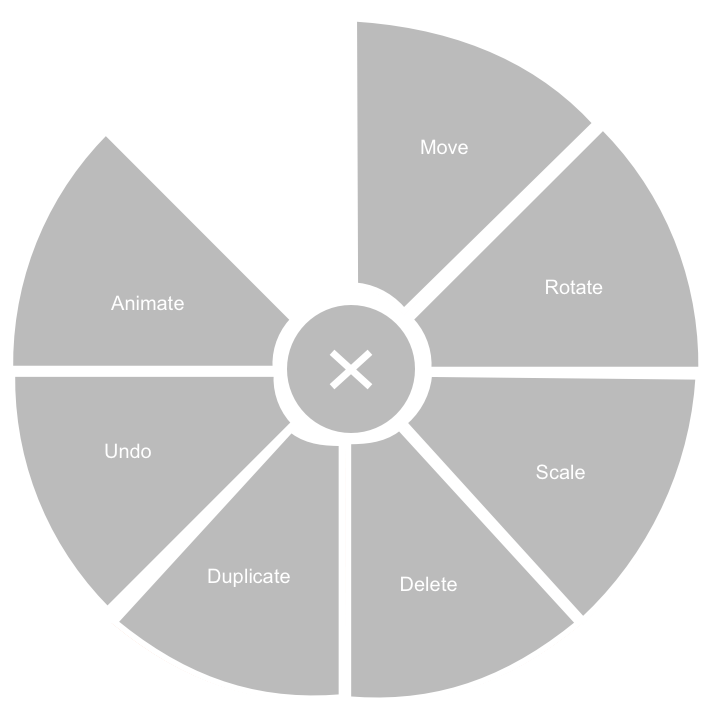
\includegraphics[width=.8\linewidth]{hi-fi/selector.png}
\caption{Digital representation of object manipulation UI}
\label{fig:hifi:selector}
\end{figure}

\begin{figure}
\begin{subfigure}{.5\textwidth}
  \centering
  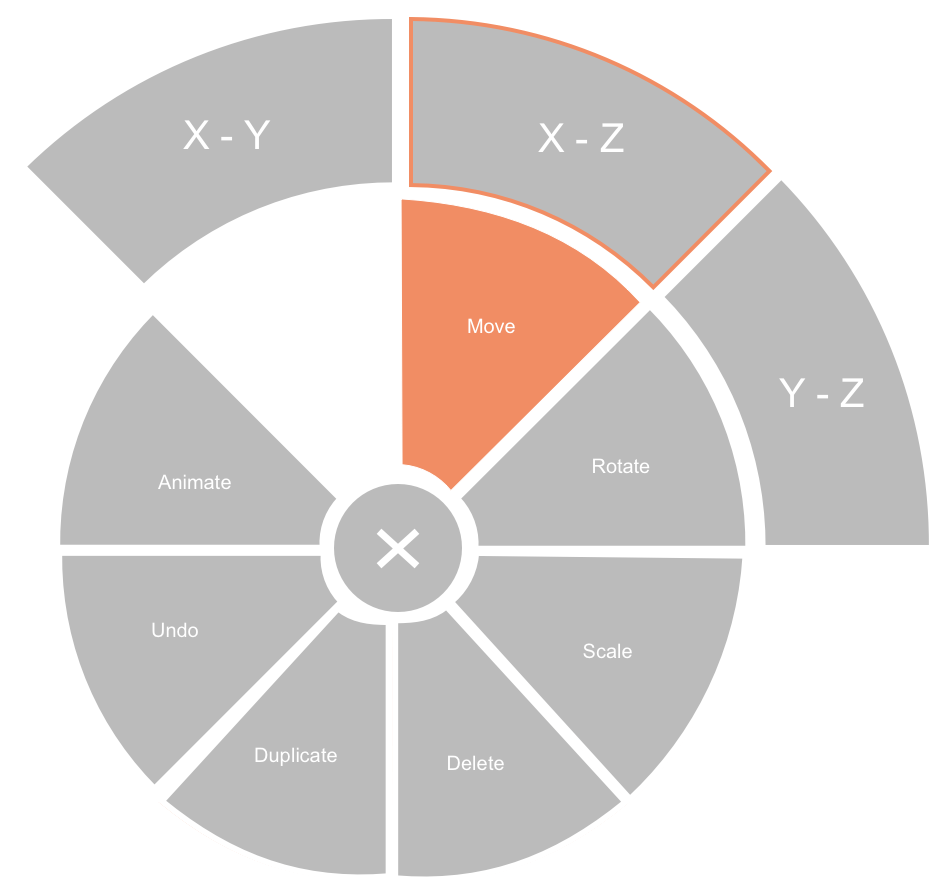
\includegraphics[width=.8\linewidth]{hi-fi/selector-submenu.png}
  \caption{Accessing a submenu of the UI}
  \label{fig:hifi:selector:select}
\end{subfigure}%
\begin{subfigure}{.5\textwidth}
  \centering
  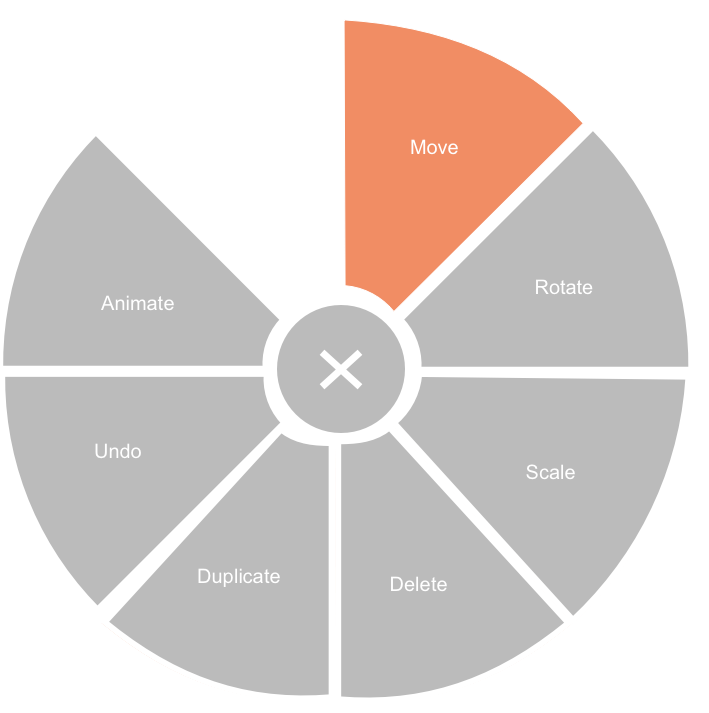
\includegraphics[width=.8\linewidth]{hi-fi/selector-select.png}
  \caption{Selection in the UI}
  \label{fig:hifi:selector:submenu}
\end{subfigure}
\caption{Multilevel UI for object manipulation}
\label{fig:hifi:selector}
\end{figure}

\subsubsection{User Input and Object manipulation}
Interactions and sequences for selecting and manipulating objects (Figures \ref{fig:hifi:scenario1},\ref{fig:hifi:scenario2},\ref{fig:hifi:scenario3} ) are explained in this section as user scenarios.
\begin{itemize}
  \item \textbf{Transportation} The user hold the touchpad of the secondary controller, which then points a raycast from the controller. The user points to a desired position and releases the touchpad to teleport to the targeted location.
  \item \textbf{Selecting an object} The user points the controller towards object, so that the raycast hits it. Then the user clicks the selection-button to select the targeted object.
  \item \textbf{Moving an object} When the user selects the object,  a selection plane becomes visible alongside the object (Figure \ref{fig:hifi:scenario:selected}). By targeting the object and holding the selection-button the user can now use the raycast to position the object along the selection plane. If the user wants to move the object in the third dimension (that is not covered by the grid), grab the grid in a similar fashion and points with the raycast to the plane that the object should be elevated/moved to. It's state is movable by default. Unless changed in the selector UI (section \ref{result:hifi:selector}), it can be moved after creation or selection. The axis' of the grid can be changed using the selector UI. The user can use the direct selection button on the secondary controller to move an object using direct selection (explained in section \ref{theory:toolsandtech:direct}).
  \item \textbf{Creating a new object} The user opens the Belt interface and selects the "New Component" button (in the hierarchy section), which displays a new view (Figure \ref{fig:hifi:beltui:add}). This view displays miniatures of objects that are avaliable to the user in the scene (figurt \ref{fig:hifi:scenario:add}). The user finds the desired object, grabs it by holding the selection-button and points in the world to deside its position. The object is placed by releasing the selection-button.
  \item \textbf{Duplicating an object} The user selects the object thats desired for duplication then opens the selector UI, then selects the 'Duplicate' option. The duplicated object is created at the current point of the raycast.
  \item \textbf{Properties of an object} The user opens the Belt UI, then selects an object with the raycast. The selection can be made on the 3D object with the raycast or on the object name in the hierarchy in the UI. When an object is selected, all properties for this object is displayed in the right section of the Belt UI (Figure \ref{fig:hifi:scenescreen}). A new property can be added by selecting a property in the "Add property" button displayed in figure \ref{fig:hifi:scenario:addprop}.
\end{itemize}

%% ********* FIELD-OF-VIEW IMAGES **********

%% BELT UI MAIN UI
\begin{figure}
  \centering
  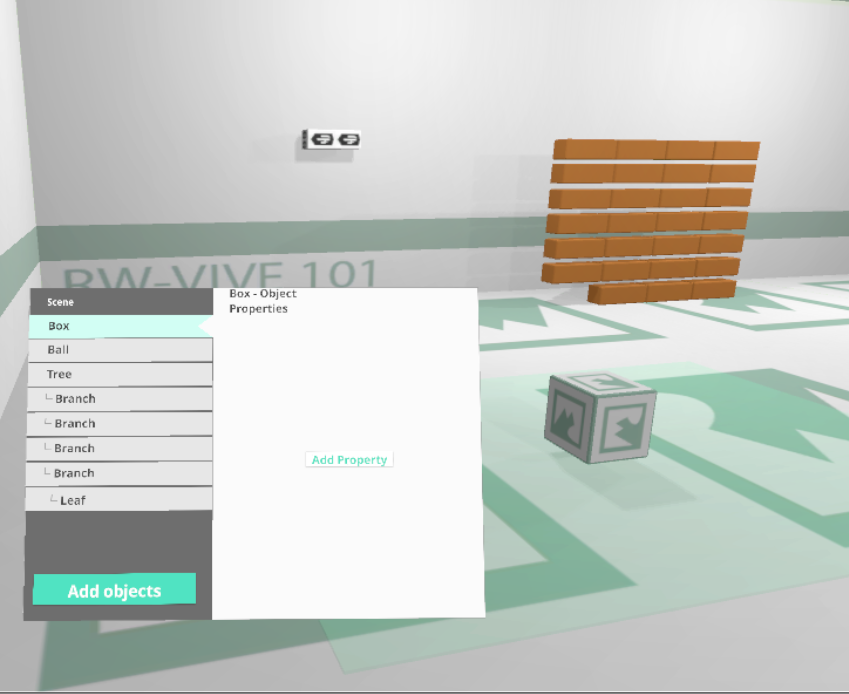
\includegraphics[width=.8\linewidth]{hi-fi/scenario-scenescreen.png}
\caption{Field of view image of the main BeltUI interface}
\label{fig:hifi:scenario2}
\end{figure}

%% OBJECT MANIPULATION AND SELECTOR
\begin{figure}
  \begin{subfigure}{.5\textwidth}
  \centering
  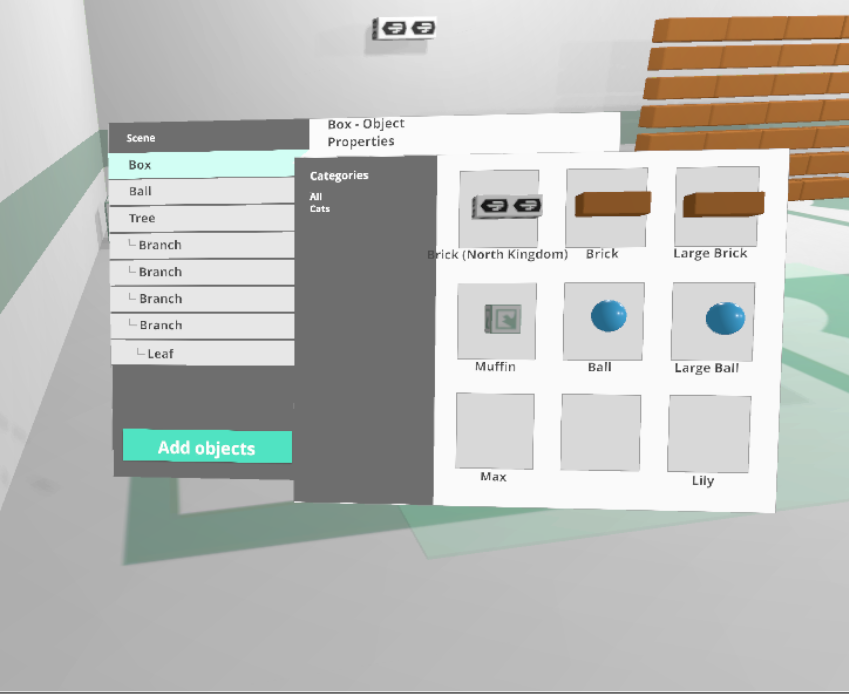
\includegraphics[width=.8\linewidth]{hi-fi/scenario-add.png}
  \caption{Interacting with piemenu on controller}
  \label{fig:hifi:scenario:selector}
  \end{subfigure}%
  \begin{subfigure}{.5\textwidth}
    \centering
    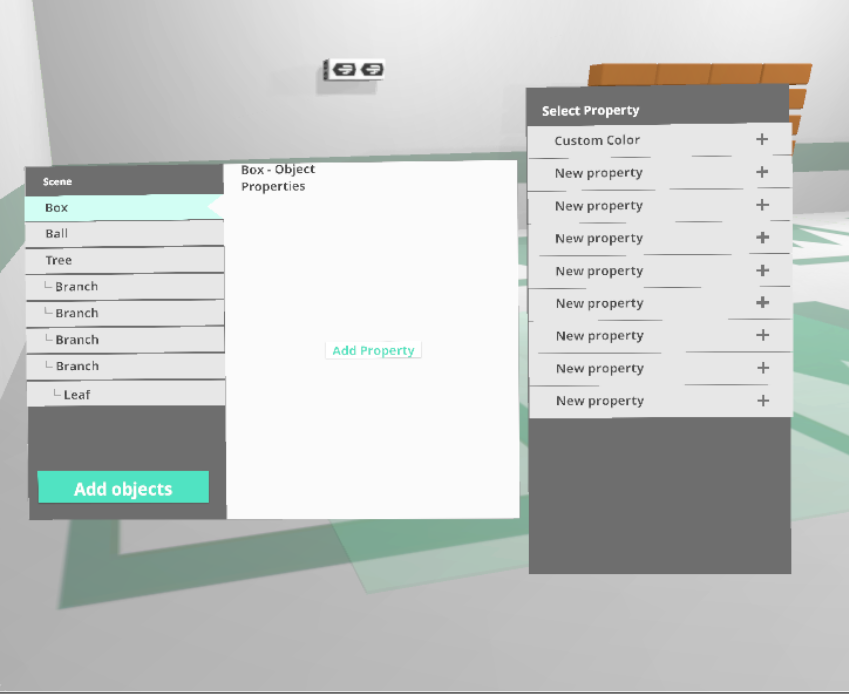
\includegraphics[width=.8\linewidth]{hi-fi/scenario-addprop.png}
    \caption{Moving an object with the raycast}
    \label{fig:hifi:scenario:move}
\end{subfigure}
\caption{Field of view image when manipulating objects}
\label{fig:hifi:scenario1}
\end{figure}

%% BELT UI EXTRA SCREENS
\begin{figure}
  \begin{subfigure}{.5\textwidth}
  \centering
  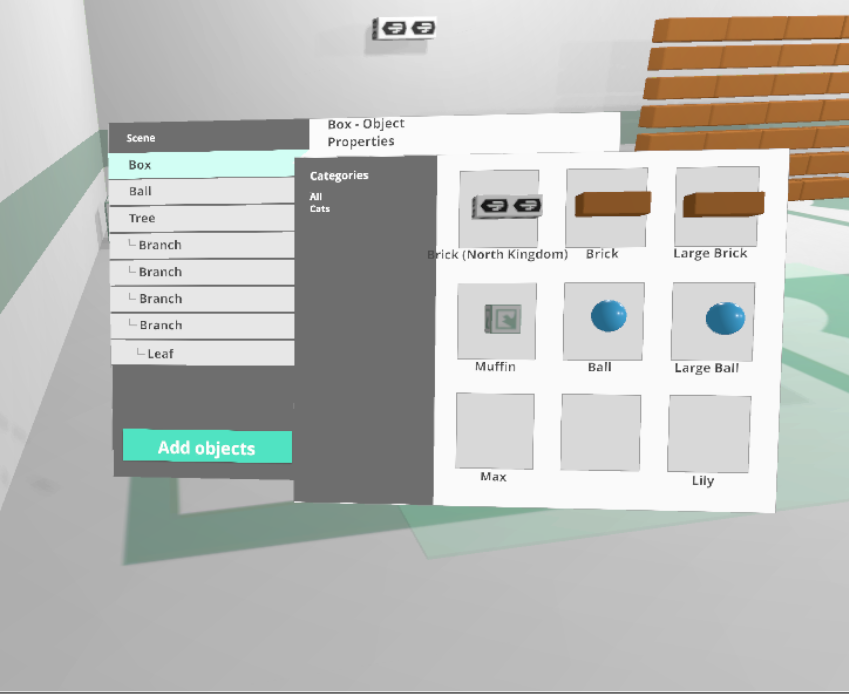
\includegraphics[width=.8\linewidth]{hi-fi/scenario-add.png}
  \caption{Creating a new object}
  \label{fig:hifi:scenario:add}
  \end{subfigure}%
  \begin{subfigure}{.5\textwidth}
    \centering
    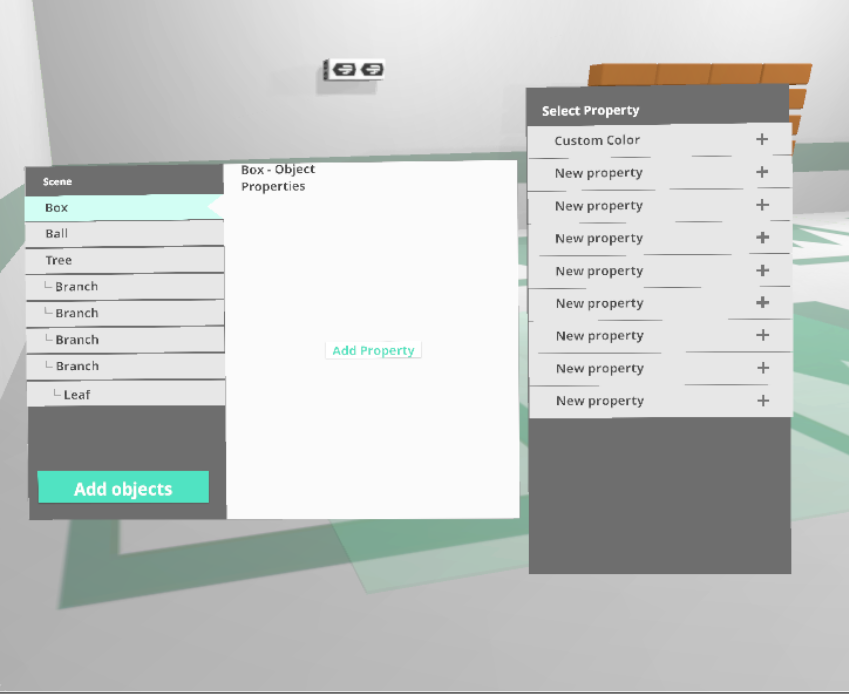
\includegraphics[width=.8\linewidth]{hi-fi/scenario-addprop.png}
    \caption{Adding a property to an object}
    \label{fig:hifi:scenario:addprop}
\end{subfigure}
\caption{Field of view image with different parts of the UI}
\label{fig:hifi:scenario1}
\end{figure}

\subsubsection{Mid-level Concept}
\label{result:hifi:midlevel}
The interviews and the hardware analysis as well as the theoretical framework in previous sections proves the validity of a mid-level solution within certain parts of the experience design process. Limited to the functionality for rough prototyping and the technical constraints, a mid-level design solution is presented. This solution has the same basic functionality as the high-level but with some limitations and changes, which are explained in this section.

\begin{itemize}
  \item The VR application is not connected to an existing VR scene, and does therefore not support altering of scenes.
  \item Objects are selected with the touchpad.
  \item The piemenu UI that is described in section \ref{result:hifi:selector} is opened by holding down the touchpad.
  \item Selecting a "slice" in the piemenu UI does not trigger the action, but changes the mode accordingly, eg. When duplicate is pressed when an object is selected the menu closes and the mode changes to duplicate. When the user points to a surface and clicks the touchpad a duplicate of the previously selected object.
  \item Moving an object requires the user to select the object (move-mode is selected as default upon selection), point to the desired position on a surface or reference plane and clicking the touchpad.
  \item Teleportation is located in the piemenu UI.
  \item There is no way to perform direct manipulation on objects.
  \item The main UI, Belt UI from section \ref{result:hifi:beltui}, Can no longer be repositioned. It will appear in the users general direction each time it is opened.

\end{itemize}

\subsubsection{Usertests and evaluation}
Common errors, habits and insights from usertests of the hi-fi prototyps are listed in this section. This data is analyzed in section \ref{discussion}.

\begin{itemize}

  \item The reference plane can hinder the user from selecting objects behind.
  \item Users cannot visually distinguish object positioning from reference plane positioning.
  \item Moving an object along the third axis (moving the reference plane) is not intuitive for users without experience or directions of usage.
  \item Placing object along the third axis by pointing at another surface causes confusion and is hard to grasp.
  \item Its hard to place object at the edge of a surface when moving the reference plane.

  \item The selected object needs to be highlighted in order to identify it.
  \item Objects can be hard to select in complex environments due to occulusion
  \item Using direct manipulation on objects is a valuable tool.
  \item Moving objects across greater distances is hard with only teleportation as transportation.
  \item Using teleportation as a tool for getting a closer look is interupting the user in their creative process.
  \item Placing objects far away is hard if the reference plane is not (close to) orthogonal relative to the user.
  \item Having objects move upon selections causes unintended movements.
  \item It's hard to place objects next to eachother without "snap-to" functionality.
  \item No way of selecting multiple objects.

  \item The pie-menu UI is practical and intuitive.
  \item The pie-menu UI needs virbration for users to interact without looking at it.
  \item Duplication on touchpad click casuses placement in unexpected places
  \item No visual feedback upon creation, duplication or deletion of an object when the user is looking at the pie-menu.

  \item Belt UI provides a comfortable workstation in a seated position.
  \item Interaction with Belt UI can cause awkward body positioning when using raycast.
  \item Text is hard to read, icons and graphics is easier to comprehend.
  \item Placing a new object causes unintentional placements.

  \item The concept is a really nice solution to the testing and manipulation problem when switching between HMD and computer screen.
  \item Users express the potential of this concept as a tool for fast prototyping in VR.

\end{itemize}
